\documentclass[11pt]{article}
\usepackage[dvips]{graphicx, color}
\usepackage{epsfig}
\usepackage{amsmath}
\usepackage{mathptmx}

\setlength{\evensidemargin}{-0.7cm}
\setlength{\oddsidemargin}{-0.0cm}
\setlength{\textwidth}{15.5cm}
\setlength{\topmargin}{-2cm}
\setlength{\textheight}{23.5cm}
\parskip 1ex    % White space between paragraphs amount
\parindent 0pt

\usepackage{html}
\usepackage[ruled]{algorithm2e}
%\usepackage{varioref}
%\usepackage[breaklinks=true,pagebackref=true]{hyperref}
%\hypersetup{colorlinks=true,urlcolor=black,citecolor=blue}

\newcommand{\red}{\color{red}}
\newcommand{\green}{\color{green}}
\newcommand{\blue}{\color{blue}}

\graphicspath{{Figures/}}

\begin{document}

\title{Flagging in CASA}
\author{Sandra Castro, Justo Gonzalez, Urvashi Rau}
\date{05 May 2012 (last modified : 6 May 2013)}
\maketitle

This memo describes the Flagger module in CASA as available from version 3.4 onwards. Section \ref{Sec:CodeDocs} gives an outline of the software implementation, section \ref{Sec:TaskTool} lists the user-documentation for the {\tt flagdata, flagcmd} tasks and the {\tt agentflagger} tool (with some examples).  Section \ref{Sec:Running} describes what various flagging modes do, with some examples and suggestions on how to use them. Section \ref{Sec:FAQ} contains a list of frequently-asked questions and their answers.

This is a living document. Details will continue to be added (with examples). Feedback is welcome.

\tableofcontents

\section{Software Documentation}

\subsection{C++ Infrastructure}\label{Sec:CodeDocs}

\subsubsection{Framework}
%{\green Link to (or copy of) Justo's documentation of the infrastructure design, 
%with links from each 'class' box/section to the relevant doxygen code-doc pages. }

\paragraph{Main Classes}

\begin{enumerate}
\item
%\htmladdnormallink{AgentFlagger}{http://www.eso.org/~scastro/ALMA/casa/active/CasaRef/agentflagger-Tool.html}:
%\htmladdnormallink{AgentFlagger}{http://casa.nrao.edu/active/docs/CasaRef/agentflagger-Module.html}:
\htmladdnormallink{AgentFlagger}{http://casa.nrao.edu/docs/CasaRef/agentflagger-Module.html}:
The top-level AgentFlagger class that connects all of the following together, and defines the C++ user-interface 
for the agentflagger.  
This is the class used by the tool layer.

%\item \htmladdnormallink{FlagDataHandler}{http://www.eso.org/~jagonzal/Flagging-3.4-Docs/html/classcasa_1_1FlagDataHandler.html} : A top level class defining the data handling interface for the flagging module. 
\item \htmladdnormallink{FlagDataHandler}{http://casa.nrao.edu/docs/doxygen/html/classcasa_1_1FlagDataHandler.html} : 
A top level class defining the data handling interface for the flagging module. 

\item The  \htmladdnormallink{FlagAgentBase}{http://casa.nrao.edu/docs/doxygen/html/classcasa_1_1FlagAgentBase.html} 
base class defines the behaviour of all flagging agents
and contains agent-level data-selection, etc.  The main functions to be implemented by derived classes are
setAgentParameters(), preProcessBuffer(), computeAntennaPairFlags() or computeRowFlags(), getReport() . 

List of available Flag Agents : 
\begin{enumerate}
\item \htmladdnormallink{FlagAgentManual}{http://casa.nrao.edu/docs/doxygen/html/classcasa_1_1FlagAgentManual.html} :  
Flag/Unflag based on data-selections.  
The only processing done by this agent is to set the flags for all data it sees to 
True if the operation is to flag, and to False to unflag. A boolean parameter
apply determines whether to flag (apply=True) or unflag (apply=False). By
default it is set to True.

\item \htmladdnormallink{FlagAgentQuack}{http://casa.nrao.edu/docs/doxygen/html/classcasa_1_1FlagAgentQuack.html} :  
Flag time-ranges at the beginning and/or end of scans. 
Uses the YYY iteration-mode. 

\item \htmladdnormallink{FlagAgentElevation}{http://casa.nrao.edu/docs/doxygen/html/classcasa_1_1FlagAgentElevation.html} : 
Flag time-ranges based on source elevation. 
Uses the YYY iteration-mode.

\item \htmladdnormallink{FlagAgentShadow}{http://casa.nrao.edu/docs/doxygen/html/classcasa_1_1FlagAgentShadow.html} : 
For each timestep, flag antennas that are shadowed by
any other antenna.  Antennas to be flagged are chosen and marked in the preProcess() stage.
Rows are flagged in computeRow(), and this agent uses the YYY iteration-mode.

\item \htmladdnormallink{FlagAgentExtend}{http://casa.nrao.edu/docs/doxygen/html/classcasa_1_1FlagAgentExtension.html} : 
Read and extend flags along specified axes, within the
current chunk.  Uses the YYY iteration-mode.

\item \htmladdnormallink{FlagAgentClip}{http://casa.nrao.edu/docs/doxygen/htmlclasscasa_1_1FlagAgentClipping.html} : 
Flag based on a clip threshold and visExpression.
Find and flag NaNs and Infs.  Uses the YYY iteration-mode. 

\item \htmladdnormallink{FlagAgentTimeFreqCrop}{http://casa.nrao.edu/docs/doxygen/html/classcasa_1_1FlagAgentTimeFreqCrop.html} : 
The TFCrop algorithm is run per
baseline, via FlagAgentTimeFreqCrop::computeAntennaPairFlags()

\item \htmladdnormallink{FlagAgentRFlag}{http://casa.nrao.edu/docs/doxygen/html/classcasa_1_1FlagAgentRFlag.html} : 
The RFlag algorithm. 
Implements multiple passes through each chunk via the  passIntermediate() and passFinal() mechanism.

\item \htmladdnormallink{FlagAgentSummary}{http://casa.nrao.edu/docs/doxygen/html/classcasa_1_1FlagAgentSummary.html} : 
Flag counts are accumulated in computeRow()
and packaged into a Record in getResult(). 

\item \htmladdnormallink{FlagAgentDisplay}{http://casa.nrao.edu/docs/doxygen/html/classcasa_1_1FlagAgentDisplay.html} : 
Visibilities are read and displayed from computeAntennaPair(). Navigation-buttons control the order in which the framework iterates through baselines. 

\end{enumerate}



\item The \htmladdnormallink{FlagReport}{http://casa.nrao.edu/docs/doxygen/html/classcasa_1_1FlagReport.html} class allows each flag agent to build and return 
information (summary counts, reports as plots, etc) to the user (and/or) to the display agent
for end-of-MS reports.
\end{enumerate}


\subsubsection{Control Flow}
%{\green  Justo, if you have a nicer way to describe the control flow, then please replace this part,  but otherwise, just this text-algorithm may be good-enough for this document (after it's completed).  If you already have the different iteration-modes explained somewhere (in one of the .h files), we can just point to it from here.  }


%%% For documentation on how to use this syntax, see the PDF file from here : 
%%  http://www.ctan.org/tex-archive/macros/latex/contrib/algorithm2e/

\begin{algorithm}
  \SetLine
%  \linesnumbered
  \dontprintsemicolon
  \vspace{0.5cm} 
  \KwData{Pre-selected Measurement Set}
  \KwIn{List of Flag Commands}
  \KwOut{Flags updated in-place + summaries/reports}
  \vspace{0.5cm} 
  {Setup FlagDataHandler :} \;
  {Build Agent List }\;
  \While (\tcc*[f]{chunks (array,obs,field,spw)}) { more chunks }
  {
    \While (\tcc*[f]{sub-chunks (ntime)}) { more times }
    {
      \ForAll (\tcc*[f]{agents}) { agents }
      {
        \If {agent touches this data}
        {
          {agent :: pre-Process current buffer}\;
             \If {iterationApproach = XXX}
             {
               \ForAll {baselines}
               {
                  {agent :: computeAntennaPairFlags()}\;
               }
             }
             \If {iterationApproach = YYY}
             {
               \ForAll {rows}
               {
                {agent :: computeRowFlags() }\;
               }
             }
        }
      }
    }
    {fdh :: Flush Flag Cube}\;
  }
  {Gather Reports from all agents} \;
\end{algorithm}





\subsubsection{Performance Optimizations}

%{\green  Explanation of various performance-optimization features  }


There are several performance-optimization choices that can be made. 
Some of these are under the users control, and some have automated heuristics.

\paragraph{List mode}

It helps to combine multiple flag commands into a single run ONLY if most of the
commands require the same data to be read.  

The goal is to read data once, apply multiple flag commands, and write flags once.

\begin{enumerate}
\item  Manual-flag commands read only meta-data.
\item  Shadow, elevation read meta-data + processing to calculate uvw, azel.
\item  Clip reads visibilities.
\item  tfcrop and rflag read visibilities and flags
\item Extend, summary read flags
\end{enumerate}



\paragraph{Data pre-selection}
If only a subset of the Measurement Set is to be traversed for flag-calculation,
it helps to pre-select and iterate through only that section of the MS.  
When multiple flag commands are supplied, with different data-selections, 
this pre-selection is calculated as a loose union of all input selection parameters
(currently a list of all unique spectral-windows and field-ids).

This is done automatically at the task level, and is in the control of the user at the 
tool level (via {\tt af.selectdata()}.

Note that there is a second level of selection per agent (command) that ensures
that each agent (command) sees only its correct subset of the data. 
The above pre-selection is purely for optimization reasons to prevent the infrastructure
from stepping through and rejecting untouched parts of the data (even though the
meta-data reads requires for the checks per chunk are minimal). 

\paragraph{Asynchronous I/O}
Asynchronous I/O is a data-access optimization that applies when iterating through the
dataset in chunks.  It uses multi-threading to pre-read the next chunk of data from disk
while the current chunk is being processed.

The user has the option of enabling asynchronous I/O by setting the following 
variables in the .casarc file. 

\begin{verbatim}
VisibilityIterator.async.enabled: true     # if present and set to false then async i/o will work
VisibilityIterator.async.nBuffers: 2       # the default value is two
VisibilityIterator.async.logFile: stderr   # Send async i/o debug log messages to this file
                                           # if not present or file is invalid then no logging occurs
VisibilityIterator.async.logLevel: 2       # Level of log messages to output (two is good, too); defaults to 1

FlagDataHandler.asyncio: true                # True : enable async-IO for the flagger (clip,tfcrop,rflag)
FlagDataHandler.slurp: true                  # True : enable ??
FlagAgent.background: true                   # True : enable threading mode
\end{verbatim}

Asynchronous I/O helps ONLY when data I/O dominates the total cost. 
For our current list of agents/algorithms, this helps only for agents that read 
visibilities. Therefore asynchronous I/O is activated only if clip or tfcrop or rflag 
are present in the flag-command list.


\paragraph{Agent parallelization}

Parallel execution of flagging agents helps when processing dominates the runtime, but there
are several factors that will affect performance. 
Parallelization by agent is helpful only if there is a list of agents of similar type, and the number of
agents is less than the number of available cores.  Parallelization by data-partitioning (chunks of
baselines, for example) is useful if all agents touch all baselines and do not require communication
across baselines).

Agent-level parallelization is currently disabled, but as part of 
\htmladdnormallink{CAS-3861}{https://bugs.nrao.edu/browse/CAS-3861}, heuristics will be implemented internally, and then documented here.



\paragraph{Interaction between Async IO and Agent parallelization}

Figures \ref{Fig:AsyncDiags} symbolically shows how async-IO and agent parallelization would scale
when IO dominates, vs when processing dominates.

\begin{figure}
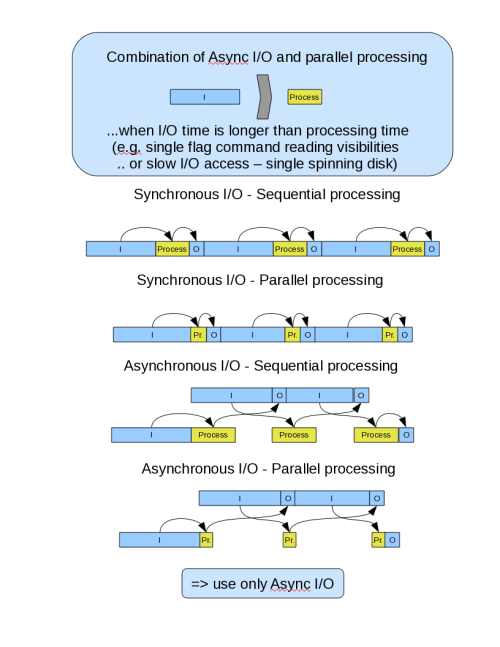
\includegraphics[scale=0.7]{async.parallel.diagram.IOdominates.png}
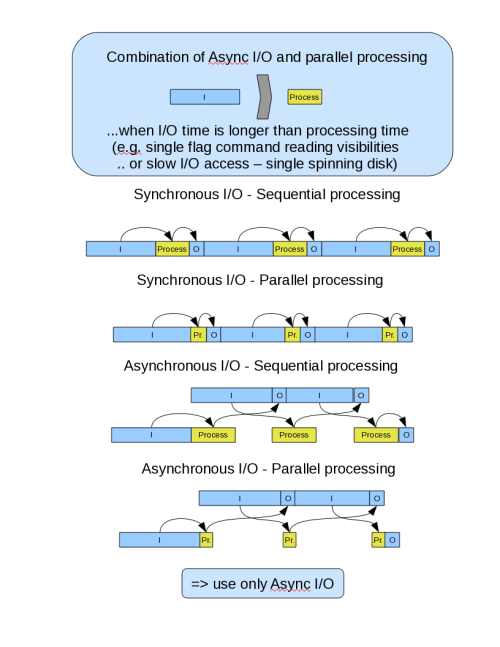
\includegraphics[scale=0.7]{async.parallel.diagram.IOdominates.png}
\caption{Explanation...}
\label{Fig:AsyncDiags}
\end{figure}






\subsubsection{Timing Tests}

Data : 

Continuum : few fat channels.\\
SpectralLine : many thin channels.\\

SinglePointing : contiguous scans on the same field\\
Mosaic  :  each scan is a different fields.\\

\begin{enumerate}
\item \label{dA} L-band continuum , Single Pointing   ----- need to decide dataset (probably G55.7+3.4\_1s.ms)
\item \label{dB} L-band spectral-line , Mosaic            ----- need to pick dataset 

\end{enumerate}


\paragraph{Comparison between modes}
%{\green Tables from Justo for 50 and 150 GB continuum datasets. }


\begin{figure}
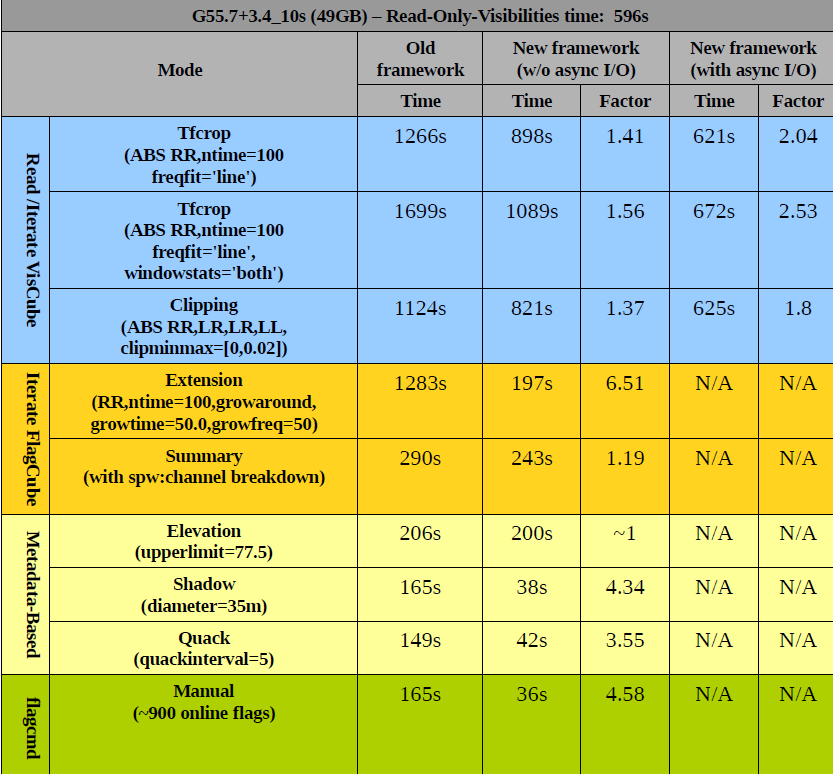
\includegraphics[scale=0.7]{table.timings.50GB.G55data.png}
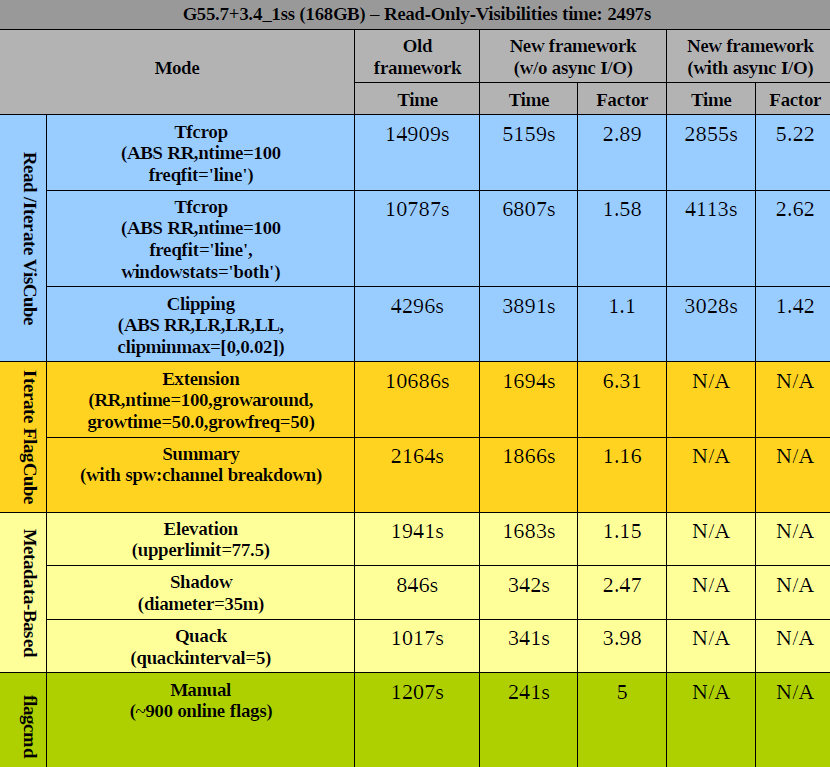
\includegraphics[scale=0.7]{table.timings.150GB.G55data.png}
\caption{These tables show timing comparisons between various modes, for two EVLA continuum datasets. Parameters of the datasets are... }
\end{figure}


\paragraph{Break-down of timings} : if possible, with and without async-IO.
\begin{enumerate}
\item  Only-reading-visibilities 
\item  Only-reading flags
\item  Only-writing flags
\item  (pls ignore if this makes no sense.) Only-iterating through the visbuffers without reading/writing anything (i.e. to see if much time is saved by the loose union). 
\end{enumerate}

\paragraph{Comparison between data-shapes and iteration patterns}

Two types of datasets : wideband continuum single-pointing,   spectral-line mosaic



%%%%%%%%%%%%%%%%%%%%%%%%%%%%%%%%%%%%%%%%%%%%%%%%%%%%
%%%%%%%%%%%%%%         SECTION           %%%%%%%%%%%%%%%%%%%%%%%%%%%
%%%%%%%%%%%%%%%%%%%%%%%%%%%%%%%%%%%%%%%%%%%%%%%%%%%%



\subsection{Python tool and task}\label{Sec:TaskTool}

\subsubsection{agentflagger tool}
\paragraph{Examples how to use the the new flagging framework from the tool.}
All the functions available in the tool are explained
\htmladdnormallink{here.}{http://www.eso.org/~scastro/ALMA/casa/active/CasaRef/agentflagger-Module.html}

\begin{enumerate}
\item Open the MS or a calibration file and attach it to the tool.

The function
takes three arguments, the MS or CAL table, the iteration approach to use and the time interval. 
Only the MS is mandatory to use. By default it will use the
FlagDataHandler::SUB\_INTEGRATION iteration approach and 0.0 seconds as the
time interval.

\begin{verbatim}
    af.open('my.ms')
\end{verbatim}

\item Select the data where to flag. If left blank, the whole MS will be
selected.

This step will use the MS Selection class. There are two functions to perform the
selection. One takes a Python dictionary (Record in C++) of the parameters, the
other takes the individual parameters as arguments.

\begin{verbatim}
  1) First method:
    selection={}
    selection['spw']="0:1~10"
    selection=['scan']="1"
    af.selectdata(selection)

  2) Second method:
    af.selectdata(spw="0:1~10", scan="1")
\end{verbatim}

\item Parse the parameters of the flagging agents.

Now it is time to build a list of the agents that we want to run to process the data. This
step will create a list of all the agents that will be executed to flag/unflag the data.
This method can be called multiple times. Every call should contain the desired parameters of
the agent and optionally data selection parameters. When data selection parameters are present,
the agent will only loop through that portion of the data.

This method will check if the requested agent (mode) is known from the following list
(manual, clip, quack, shadow, elevation, tfcrop, rflag, extend, unflag and summary). If
empty or unknown, it will give a warning and return.

If any tfcrop, rflag or extend mode is present, this method will calculate the maximum value
of time interval (ntime) from these agents. The maximum value will be used for
all the agents in the list.

A similar situation will happen with the combinescans parameter. If any of the combinescans is
True, it will be taken as True to all agents.

Async I/O will be activated if any of the modes clip, tfcrop or rflag is requested.

Only for the tfcrop agent, if a correlation ALL is requested, this method will create one
agent for each available polarization in the MS. For example, if the MS contains polarizations
XX and YY and the parameter is correlation="ABS\_ALL", then there will be two
tfcrop agents, one with correlation="ABS\_XX" and the other with
correlation="ABS\_YY". The apply parameter is set by default to True to apply
the flags.

\begin{verbatim}
     agent_pars = {}
     agent_pars["mode"] = "clip"
     agent_pars["clipzeros"] = true
     agent_pars["apply"] = true
     af.parseagentparameters(agent_pars)

     agent_pars = {}
     agent_pars["mode"] = "manual"
     agent_pars["autocorr"] = true
     af.parseagentparameters(agent_pars)

     agent_pars = {}
     agent_pars["mode"] = "summary"
     agent_pars["basecnt"] = true
     af.parseagentparameters(agent_pars)
\end{verbatim}

There are convenience functions to parse the agent's parameters, one specific for each agent.
The above calls can be done instead using these functions.

\begin{verbatim}
     af.parseclipparameters(clipzeros=true, apply=true)
     af.parsemanualparameters(autocorr=true)
     af.parsesummaryparameters(basecnt=true)
\end{verbatim}

In either one of the cases, three agents will be created. We need to initialize the agents, which
will call the constructor of each one of them and set the parameters that were given in the previous
calls. Some basic checks will be performed at this stage for types and values of the parameters.

If any tfcrop, rflag, extend or display agent is in the list, the iteration approach will be
set to a different value depending on whether combinescans is true or not. When True, the
iteration approach will be set to
FlagDataHandler::COMBINE\_SCANS\_MAP\_ANTENNA\_PAIRS\_ONLY, otherwise to
FlagDataHandler::COMPLETE\_SCAN\_MAP\_ANTENNA\_PAIRS\_ONLY.

\item Initialize the agents.

This method will create agents and add them to a FlagAgentList. If for any reason, the call to
FlagAgentBase::create(fdh\_p, agent\_rec) fails, an error message will be
displayed. Any agents previously added to the FlagAgentList will remain there. A subsequent call to this method can be done to add
more agents to the same FlagAgentList.

\begin{verbatim}
     af.init()
\end{verbatim}

\item Process the flags and write them to the MS.

The run method takes two parameters, writeflags and sequential.
The parameter writeflags controls whether to write the flags or not to the MS.
By default it is set to True. Setting writeflags to False is useful when one
wants to run the tool together with the display agent to see what is going to be
flagged before deciding to write or not to the MS. The sequential parameter
controls if the order of the agent's list is to be preserved or not. If set to
False, the order will not be preserved and the framework may execute the agent's list in parallel.
By default sequential is set to True.

The run method gathers several reports, depending on wich agents are run. The display and summary agents
produce reports that can be retrieved from calling the run method. The reports are returned via a Python
dictionary. When executed from the task, only the report of the
last summary in the list will be returned. If executed from the tool level,
multiple reports are allowed for the summary agent.

In the previous example, only one summary agent was added to the list, therefore
two reports will be returned in the dictionary. The first report contains the
summaries per field, spw, scan, correlation, etc. The second report
gives the antenna positions for plotting.

\begin{verbatim}
     my_reports = af.run()
\end{verbatim}

\item Destroy the tool.

\begin{verbatim}
    af.done()
\end{verbatim}
 \end{enumerate}
 
\paragraph{The following are only possible in the tool.}
\begin{enumerate}

\item Run multiple summary agents in a list. In order to do this, add as many
summary agents are desired when parsing the agent's parameters. You can do this by
calling the af.parseagentparameters() several times before calling af.init().

\item Determine to run the agents in sequential or in parallel. Set the
'sequential' parameter of the run method to True or False to control this.

\item Flag CAL tables in currently only possible in the tool. Give a CAL table
name when calling the af.open() method instead of a MS.

\end{enumerate}

\paragraph{Explain the heuristics applied for the automatic activation of async
I/O and parallel run}

\subsubsection{flaghelper functions}

This Python file contains many helper functions for flagdata and flacmd. The
functions can be imported inside casapy.

\begin{verbatim}
     import flaghelper as fh
\end{verbatim}

\subsubsection{flagdata task}
Help for the flagdata task is available \htmladdnormallink{here.}
{http://casa.nrao.edu/docs/taskref/flagdata-task.html}

\subsubsection{flagcmd task}
Help for the flagcmd task is available \htmladdnormallink{here.}
{http://casa.nrao.edu/docs/taskref/flagcmd-task.html}



%%%%%%%%%%%%%%%%%%%%%%%%%%%%%%%%%%%%%%%%%%%%%%%%%%%%




\section{Running the flagger}\label{Sec:Running}

\htmladdnormallink{These slides}{http://www.aoc.nrao.edu/~rurvashi/DataFiles/Talk_FlaggingCASA3.4.pdf}
summarize the CASA flagger infrastructure and user-options.

\htmladdnormallink{Task Documentation}{http://casa.nrao.edu/docs/TaskRef/TaskRef.html}
\htmladdnormallink{Tool Documentation} {http://casa.nrao.edu/docs/CasaRef/CasaRef.html}

%%%%%%%%%%%%%%%%%%%%%%%%%%%%%%%%%%%%%%%%%%%%%%%%%%%%

\subsection{Single flag mode (flagdata)}

All the following flagging modes operate on user-specified subsets of the data.
The dataset is iterated-through in chunks consisting of one field, one spw, and a
user-defined timerange (default is one scan). 
Modes that read visibilities also respond to some simple expressions that are applied to 
the visibilities, before they are considered for flagging 
(for example, $ABS\_RR,LL,  ABS\_I, REAL\_V,  ABS\_ALL$).

\subsubsection{Manual Flag/Unflag}

Selection-based flagging and unflagging can be done via the \htmladdnormallink{MSSelection syntax}{http://www.aoc.nrao.edu/~sbhatnag/misc/msselection/msselection.html}.  
This flagging mode is meant for marking subsets of the data that are known to be
unfit for calibration or imaging. Some examples are online flags from the data-recording system, known frequency ranges 
with strong RFI, etc. It is also possible to use the parameter 'autocorr' to
flag only auto-correlations in the MS.

\subsubsection{Quack}

Data at scan edges can sometimes be unusable for some antennas or baselines (for example, if some antennas take longer 
than others to slew to a new target, but the signal correlation and recording starts before all antennas are ready), and it 
is often useful to flag these edges.The 'quack' mode allows the user to specify time-ranges from the beginning and/or end of 
all selected scans. 

\subsubsection{Elevation}

Data taken when the antennas are pointed at low elevations can sometimes be unusable and require flagging.  Reasons for 
flagging data at low elevations include increased shadowing between antennas, increased sensitivity to RFI from the horizon, 
elevation-dependent antenna-gain variations, corrupted spectra due to looking
through a longer path-length through the atmosphere, etc.  At high elevations, one problem could be increased pointing 
errors when an Alt-Az antenna tracks a source near the Zenith. The 'elevation'
mode allows the user to specify elevation-ranges to be flagged, for the selected data.

\subsubsection{Clip}

Strong outliers can be flagged using a simple threshold (range). If a valid data
range is known $a-priori$, clipping can be done as the first step before basic calibration or other editing.
The 'clip' mode allows the user to specify a range, and clip all values either within or outside the range. 
Values are defined as expressions that involve data columns and
correlation-selections (for example, ABS\_I or REAL\_RR,LL, etc).
NaNs and Infs are always included in the clipping. By default, if no range for
clipping is given, it will flag only NaNs and Infs. Optionally, exact zeros can
flagged using the clipzeros parameter. Early EVLA data-sets occasionally have
exact zeros in parts of the data where the backend-system is overloaded, and NaNs and Infs have sometimes been 
reported when data is converted between packages and formats.


\subsubsection{Shadow}

Shadow flags are computed by considering the positions and diameters of a list of antennas
along with the target direction at each timestep.  
All antennas present in the ANTENNA subtable of the MS as well as any other positions 
and diameters supplied via an external file are considered for shadow-flag calculations. 

Shadow flags are computed as follows (for every timestep): 
\begin{enumerate}
\item Calculate or read the $u,v,w$ values (in meters) for all possible antenna-pairs, 
using the phase-reference center of the observation to define the pointing-direction. 
The values of $u,v,w$ are re-used when already present in the MS, and calculated only for
baselines without visibilities in the current timestep (to account for antennas that did not produce
data for that timestep, but were still physically present and creating shadows).

\item For each possible antenna pair, use the value of $w$ to determine which antenna is behind and
which is in front ( $w<0$: antenna 1 is behine antenna 2 ).  

\item Mark the 'behind' antenna for flagging
if $\sqrt{u^2+v^2} < r_1 + r_2 - tol$. Here,  $r_1,r_2$ are the radii of the two antennas, and $tol$ is
the amount (in meters) of allowed shadowing before being marked for flagging. 
\end{enumerate}


\begin{figure}
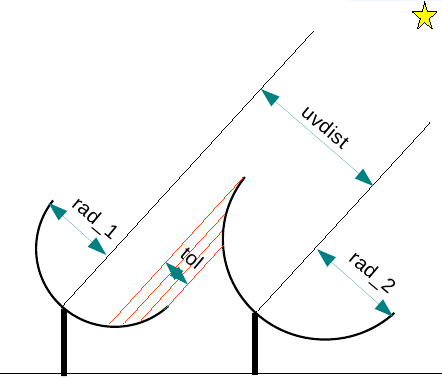
\includegraphics[scale=0.7]{shadow.diagram.png}
\caption{This figure shows the geometry used to compute shadowed antennas.}
\end{figure}



Note : The use of the phase-reference center as the pointing-direction for all antennas, is accurate in most 
cases, but will be approximate during on-the-fly mosaicing. However, since it is unlikely that an 
on-the-fly mosaic will be done with only one phase-reference center on a large-enough field-of-view
for shadow-flag differences to become significant.  


Note : Antennas that are not part of the MS ANTENNA subtable can be included in the calculation of
shadow flags by specifying a list of positions and diameters in an external file.   Note however that
the calculations will not account for the fact that antennas not part of
the observation, but still physically present on the ground, may not be pointing in the same direction as all the others
(as is assumed in the calculations).  If desired, the antenna diameters in the external file could
be adjusted accordingly.

Example : 
\begin{verbatim}
name=VLA1
diameter=25.0
Position=[-1601144.96146, -5041998.01971, 3554864.76811]

name=VLA2
diameter=25.0
position=[-1601105.76646, -5042022.39178, 3554847.24515]
\end{verbatim}

A helper-function has been provided to construct this list from an MS (possibly a different dataset)
that contains the required information in its ANTENNA subtable.

\begin{verbatim}
import flaghelper;
antlist =  flaghelper.extractAntennaInfo (
            msname='shadowtest.ms',
            antnamelist=['VLA1','VLA2','VLA9','VLA10'] );
flaghelper.writeAntennaList('antlist.txt',antlist);
\end{verbatim}


Figure \ref{ShadowExample} shows the flagging results from a simulated observation that spans a large
elevation range. Antennas near the center of the array are shadowed more than the others (left plot). 
If some antennas are split-out of the dataset, the ANTENNA subtable will have fewer antennas, and the shadow
flags will change (middle plot).  However, by specifying the positions and diameters of the missing antennas
via the external file, the correct shadow flags are recovered (right plot). 

\begin{figure}
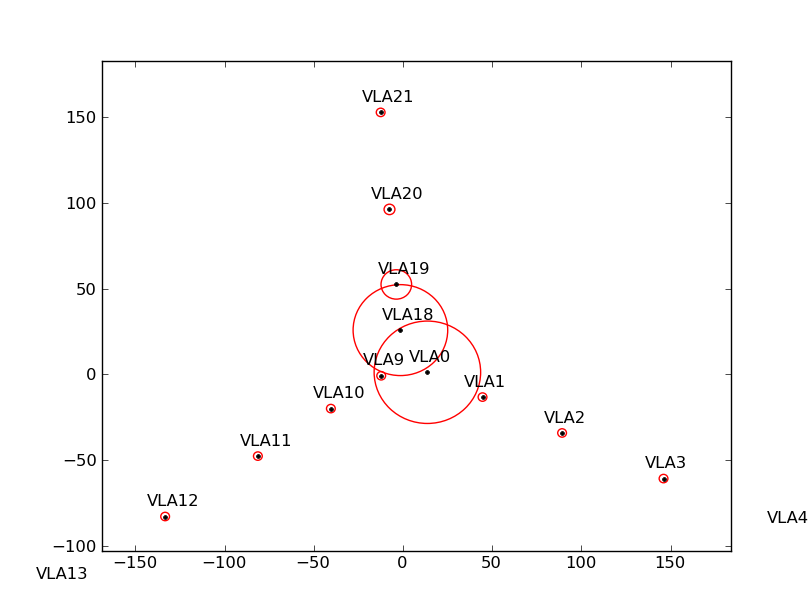
\includegraphics[scale=0.5]{plot.allants.shadow.png}
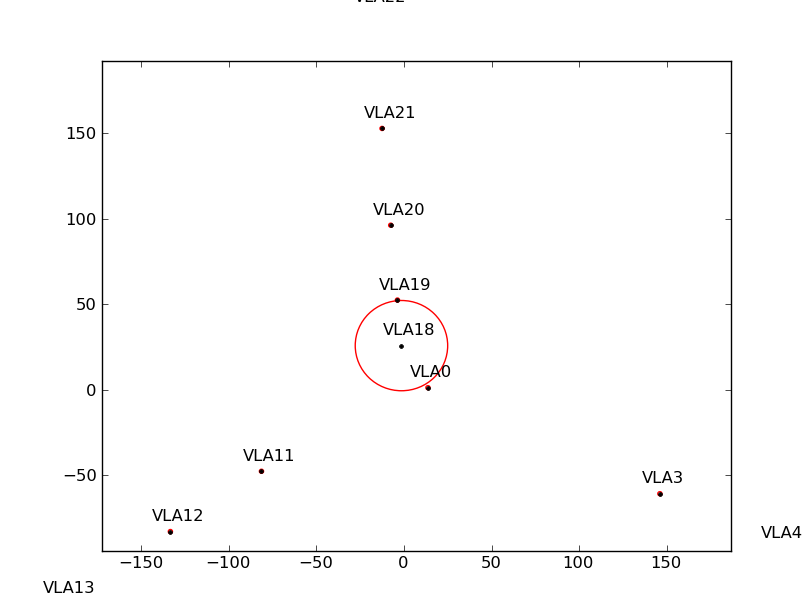
\includegraphics[scale=0.5]{plot.someants.shadow.png}
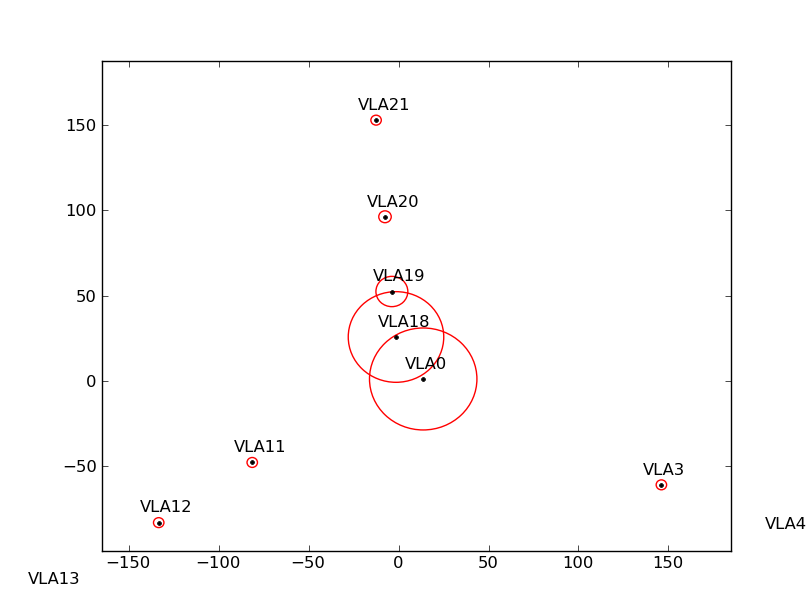
\includegraphics[scale=0.5]{plot.someants.withlist.shadow.png}
\caption{This figure shows  fractions of data flagged per antenna, for
three different use-cases. The size of the circle is proportional to the fraction of data flagged.
(LEFT) : Shadow-Flags with all antennas present in the MS,   (MIDDLE) : Shadow-Flags with four antennas (and their baselines) deleted from the MS,    (RIGHT) : Shadow-Flags from the MS with the missing antennas, but with the positions and diameters of the missing antennas specified via an external text file. The flags produced are the same as when all antennas are present in the MS.}
\label{Fig:ShadowExample}
\end{figure}


\subsubsection{TFCrop}

TFCrop is an autoflag algorithm that detects outliers on the 2D time-frequency plane, and 
 can operate on un-calibrated data (non bandpass-corrected).

The original implementation of this algorithm is described in 
\htmladdnormallink{NCRA Technical Report 202}{http://ncralib1.ncra.tifr.res.in:8080/jspui/handle/2301/127} (Oct 2003)


The algorithm iterates through the data in chunks of time.
For each chunk,  the result of user-specified visibility-expressions 
are organized as 2D time-frequency planes, one for each baseline 
and correlation-expression result, and the following steps are performed.

\begin{enumerate}
\item Calculate a bandshape template : 
Average the data across time, to construct an average bandpass.
     Construct an estimate of a clean bandpass (without RFI) via a
     robust piece-wise polynomial fit to the average bandpass shape.

       Note : A robust fit is computed in upto 5 iterations. 
It begins with a straight line fit across the full range, and gradually increases to 
     'maxnpieces' number of pieces with third-order polynomials in each piece. 
At each iteration, the stddev
                                between the data and the fit is computed, values beyond N-stddev are flagged,
                                and the fit and stddev are re-calculated with the remaining points.
                                This stddev calculation is adaptive, and converges to a value that reflects 
                                only the data and no RFI.  
At each iteration,  the same relative threshold is applied to detect flags, and this results in
a varying set of flagging thresholds,  that allows deep flagging only when the fit represents the true data best.
 Iterations stop when the stddev changes 
     by less than 10\%, or when 5 iterations are completed.

     The resulting clean bandpass is a fit across the base of RFI spikes.

\item  Divide out this clean bandpass function from all timesteps in the current chunk.  
Now, any data points that deviate from a mean of 1 can be considered RFI.  This step 
helps to separate narrow-band RFI spikes from a smooth but varying bandpass, in
situations where a simple range-based clipping will flag good sections of the bandpass.

\item Perform iterative flagging (robust flagging) of points deviating from a value of 1.  

  Flagging is done in upto 5 iterations. 
   In each iteration, for every timestep, calculate the stddev of the bandpass-flattened data, flag all points further than N times stddev from the fit, and recalculate the stddev.
 At each iteration,  the same relative threshold is applied to detect flags.
     Optionally, use sliding-window based statistics to calculate additional flags.

\item Repeat steps 1 and 3, but in the other direction (i.e. average the data across frequency,
     calculate a piece-wise polynomial fit to the average time-series, and find flags
     based on deviations w.r.to this fit.)

\end{enumerate}

The default parameters of the tfcrop implementation are optimized for strong narrow-band RFI.
With broad-band RFI, the piece-wise polynomial can sometimes model it as part of the
band-shape, and therefore not detect it as RFI.  In this case, reducing the maximum number 
of pieces in the polynomial can help.     This algorithm usually has trouble with
noisy RFI that is also extended in time of frequency, and additional statistics-based
flagging is recommended (via the 'usewindowstats' parameter). It is often required to
set up parameters separately for each spectral-window.

If frequency ranges of known astronomical spectral lines are known $a-priori$, they can
be protected from automatic flagging by de-selecting those frequency-ranges via the 
'spw' data-selection parameter. 

\underline{NOTE:} It is usually helpful to extend the flags along time,
frequency, and correlation after running tfcrop. By default, the flags are extended
if more than 50\% of the timeranges are already flagged, 80\% of the
channels are already flagged and it also extends the flags to the other
polarizations in the selection. This automatic extension of flags is done
through the parameter 'extendflags'. The user has the option to fine-tune
the extension of flags via the mode='extend'
within the same flagging run such as in the example below:

\begin{verbatim}
Example :
  cmd=["mode='tfcrop' freqcutoff=3.0 usewindowstats='sum' extendflags=False ",
       "mode='extend' extendpols=True growtime=50.0 growaround=True"] 
     
  flagdata(vis, mode='list', inpfile=cmd)

\end{verbatim}

Below are some examples that demonstrate what the algorithm does with different types
of RFI.


\begin{figure}
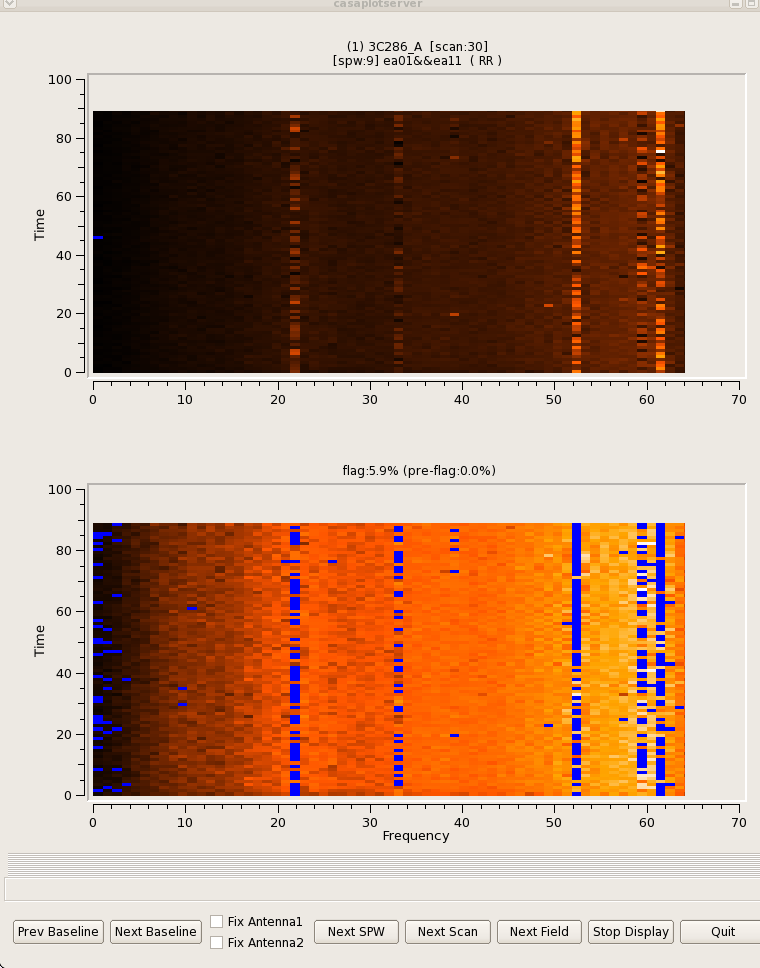
\includegraphics[scale=0.4]{flag.protect.specline.1.png}
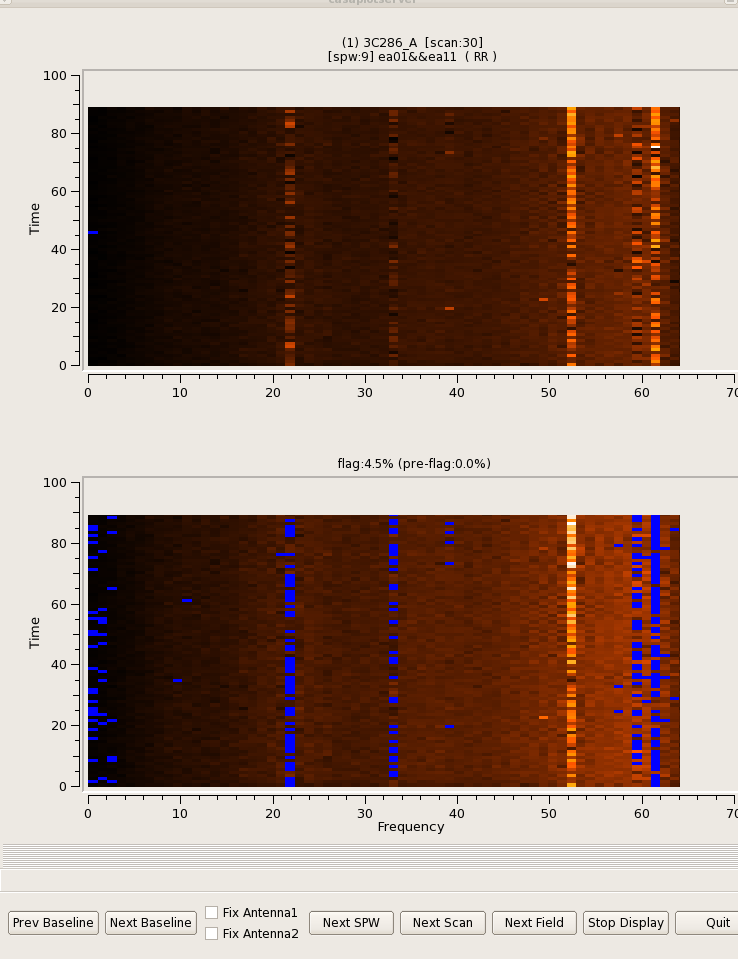
\includegraphics[scale=0.4]{flag.protect.specline.2.png}
\caption{LEFT : This screenshot represents a run where 'tfcrop' was run on a spw='9' with mainly narrow-band RFI.  RIGHT : An example of protecting a spectral line (in this case, demonstrated on an RFI spike) by setting the spw-selection to spw='0:0~45;53~63'.   In both figures, the top row indicates the data before flagging, and the bottom row after flagging.}
\end{figure}

{\red
FIG2 : Broad-band RFI
}


\subsubsection{RFlag}

RFlag is an autoflag algorithm based on a sliding window statistical filter (E.Greisen, AIPS, 2011).

The RFlag algorithm was originally developed by Eric Greisen in AIPS (31DEC11). \\
AIPS documentation : Subsection E.5 of the AIPS cookbook (\htmladdnormallink{Appendix E : Special Considerations for EVLA data calibration and imaging in AIPS}{http://www.aips.nrao.edu/cook.html#CEE})

In RFlag, the data is iterated-through in chunks
of time, statistics are accumulated across time-chunks, thresholds are calculated
at the end, and applied during a second pass through the dataset. 

The CASA implementation also optionally allows a single-pass operation where statistics
and thresholds are computed and also used for flagging, within each time-chunk
(defined by 'ntime' and 'combinescans'). 

For each chunk, calculate local statistics, and apply flags based on user supplied 
(or auto-calculated) thresholds.

RFlag mixes the data from the parallel and cross-hand correlation products to determine 
the flagging thresholds, and then it applies these common thresholds to all the correlation products. 
The parallel-hand correlation products typically have higher ranges than the cross-hand correlation 
products, and they dominate the algorithm that determines the thresholds, thus the thresholds are 
rarely hit by the cross-hand correlation product ranges. The usual way to proceed is to run RFlag 
using only the parallel-hand correlation products and then extend it to the cross-hand correlation 
products to obtain the correct results.

\begin{enumerate}
\item Time analysis (for each channel)
\begin{enumerate}
\item Calculate local rms of real and imag visibilities, within a sliding time window
\item Calculate the median rms across time windows, deviations of local rms from
                              this median, and the median deviation 
\item Flag if local rms is larger than timedevscale x (medianRMS + medianDev)
\end{enumerate}
\item Spectral analysis (for each time)
\begin{enumerate}

\item Calculate avg of real and imag visibilities and their rms across channels
\item Calculate the deviation of each channel from this avg, and the median-deviation
\item Flag if deviation is larger than freqdevscale x medianDev
\end{enumerate}

\end{enumerate}

%{\red Add info about how to use 'writeflags' + 'display' + output thresholds,
% etc...}

Reports and plots are generated from rflag (when action='calculate'), to display
the mean deviations for each channel, as well as the mean variance of 
local statistics from this median deviation (local statistics are computed in a 
sliding-window). 


Below are some examples. 

\begin{enumerate}

\item Calculate thresholds automatically per scan, and use them to find flags.
Specify scale-factor for time-analysis thresholds, use default for frequency.

\begin{verbatim}
   flagdata('my.ms', mode='rflag',spw='9',timedevscale=4.0)
\end{verbatim}
 
\item  Supply noise-estimates to be used with default scale-factors. 
  
\begin{verbatim}
   flagdata(vis='my.ms', mode='rflag', spw='9', timedev=0.1, freqdev=0.5);
\end{verbatim}

\item Two-passes. This replicates the usage pattern in AIPS.

-- The first pass saves commands in output text files, with auto-calculated thresholds.
Thresholds are returned from rflag only when action='calculate' (writing to
the MS is off).
The user can edit this file before doing the second pass, but the python-dictionary 
structure must be preserved.

-- The second pass applies these commands (action='apply').

\begin{verbatim}
  flagdata(vis='my.ms', mode='rflag', spw='9,10', timedev='tdevfile.txt',freqdev='fdevfile.txt', action='calculate')
  flagdata(vis='my.ms', mode='rflag', spw='9,10', timedev='tdevfile.txt',freqdev='fdevfile.txt', action='apply')
\end{verbatim}
            
\end{enumerate} 


\begin{figure}
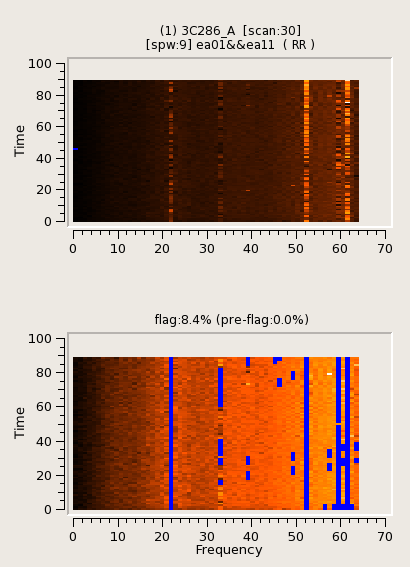
\includegraphics[scale=0.8]{rflag.before.after.png}
\caption{Example of rflag on narrow-band RFI}
\end{figure}

% {\red Add figures of the new report plots.}


\underline{NOTE:} It is usually helpful to extend the flags along time,
frequency, and correlation in a second step, after running rflag. By default, 
the flags are extended
if more than 50\% of the timeranges are already flagged, 80\% of the
channels are already flagged and it also extends the flags to the other
polarizations in the selection. This automatic extension of flags is done
through the parameter 'extendflags'. The user has the option to fine-tune
the extension of flags via the mode='extend'
within the same flagging run such as in the example below:

\begin{verbatim}
Example :
  cmd=["mode='rflag' freqdevscale=3.0 extendflags=False ", 
       "mode='extend' extendpols=True growtime=50.0 growaround=True"]
     
  flagdata(vis, mode='list', inpfile=cmd)

\end{verbatim}



\subsubsection{Extend}

Flags can be extended along various axes (within one spw, field, and time-chunk). 
Autoflag algorithms on their own often leave out pieces of RFI-affected data, in-between flagged
points, and flag extensions are often useful.  Data points can be flagged if more than half of 
the surrounding points are already flagged.  If a timerange or frequency-range is more than 
(for example) 50\% flagged, the entire range can be flagged.  Flags can be extended across
correlations, in cases where the RFI-signal-to-noise ratio is higher in some correlations where
it is easier to detect than in other correlations. 

\begin{figure}
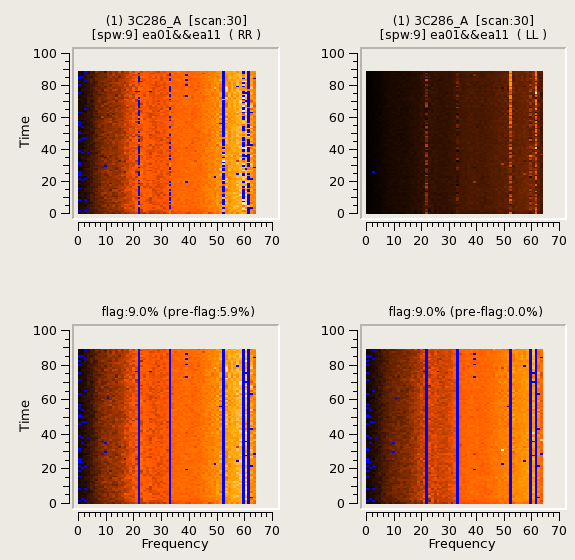
\includegraphics[scale=0.8]{flag.extension.png}
\caption{This screenshot represents a run where 'tfcrop' was run only on
'ABS\_RR' (top row) and followed by an extension along time and correlations
(bottom row). }
\end{figure}


%%%%%%%%%%%%%%%%%%%%%%%%%%%%%%%%%%%%%%%%%%%%%%%%%%%%
%%%%%%%%%%%%%%%%%%%%%%%%%%%%%%%%%%%%%%%%%%%%%%%%%%%%


\subsection{List of flag commands (flagdata, flagcmd)}
\label{Sec:FlagCmdLists}
There are two flagging tasks in version 4.0 of CASA. The main task flagdata is
a replacement for the old flagdata/flagdata2/testautoflag/flagautocorr. This
task can take parameters input from the interface as well as input from an
external text file or a list of strings. This is the so-called list mode. All the flagging commands
that apply to an MS can be combined into one single text file and read in for
processing. Similarly, the flagging commands can be written in a Python list of strings
and passed in the command line to the task. Only the summary mode is not allowed in list mode to avoid
confusion when several summaries are present in the list. The user can run
flagdata separated to get the summary of the list. 

The other task, flagcmd is a replacement for the previous version of flagcmd. It
has a re-factored interface and it can do much more than the previous version.
All the flagging modes available in flagdata are also allowed in flagcmd
(except again for the summary mode). Several input modes are available: table,
list and xml. Actions to perform on the input are: apply, unapply, list,
clear, plot and extract.

\subsubsection{Apply/ un-apply}
It is possible to truly unapply flag commands in flagcmd. In order to guarantee that only the data selected in 
the commands is unapplied, the framework will first unapply the selected rows
and then re-apply the overlapping data that got unapplied in the first pass. This is a true unapply action, but it will take longer to
process because it will re-apply all the remaining commands that have the
column APPLIED set to True inside the FLAG\_CMD sub-table of the MS.

\subsubsection{Using flag-commands in the flagcmd task}
Flag commands can be given as input to the flagcmd task in several ways. The
default is the 'table' which will have the flag commands inside the FLAG\_CMD
sub-table of the MS in a column called COMMAND.

The other input, as already detailed above is the 'list' mode, which will have
the flag commands in a text file or from a list of strings.

The 'xml' input is meant to be used for the online flags from the Flag.xml file
in the MS. It also assumes that the Antenna.xml file is present.

For all the input modes, the action='list' can be used to list the flags
commands on the screen and optionally to save them to an external output file
when the parameter savepars is set to True.

When the action='apply' is used in the inpmode table, the flags will be applied
to the MS and the APPLIED column will be updated to True. On the other hand,
when action='unapply' the APPLIED column will be set to False for all selected
table rows.

\paragraph{Examples}

\begin{enumerate}
\item Input commands from the FLAG\_CMD sub-table. 

\begin{figure}
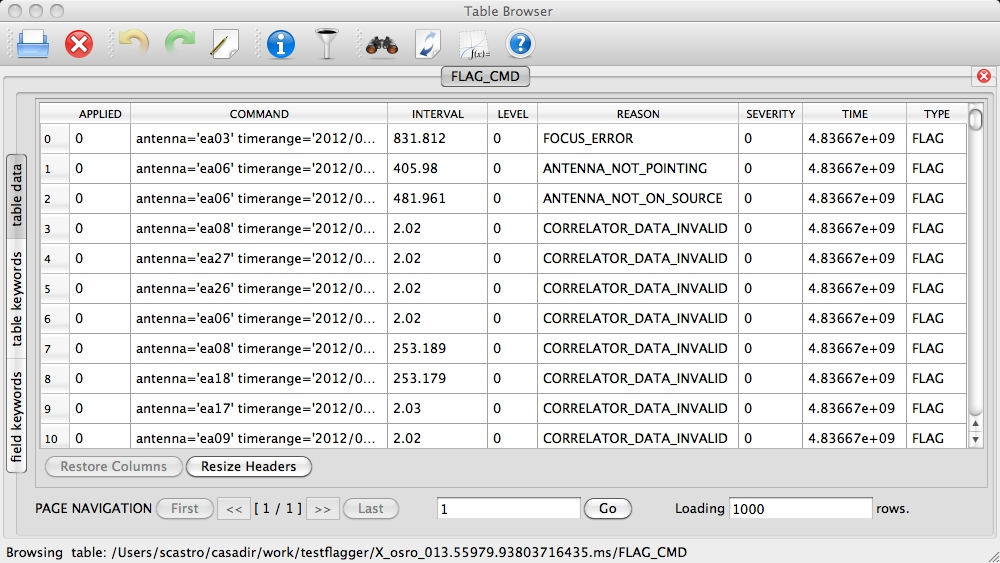
\includegraphics[scale=0.8]{flagcmd_screenshot.png}
\caption{Screenshot of the FLAG\_CMD sub-table of a MS with flag commands for the
online flags. }
\end{figure}

\begin{verbatim}
# Apply only the flag commands that contain reason='CORRELATOR_DATA_INVALID'.
The default action for flagcmd is to apply the flag commands from a table input,
therefore it is not necessary to specify inpmode='table' and action='apply'.

 flagcmd(vis='uid.ms', reason='CORRELATOR_DATA_INVALID')
  
\end{verbatim}

\item Input commands from an ASCII file.
\begin{verbatim}
# Create an input text file with all the flag commands to apply to the MS.
> cat flags.txt
 mode='manual' autocorr=True
 mode='shadow'
 mode='clip' clipminmax=[0,2] clipzeros=True correlation='ABS_ALL'
 mode='tfcrop' spw='9' correlation='ABS_YY' ntime=51.0
 mode='extend' extendpols=True

# Pass the input to the task
  flagcmd(vis='uid.ms', inpmode='list', inpfile='flags.txt', action='apply')
 
\end{verbatim}

\item Input commands via a list of strings.
\begin{verbatim}
# Give the flagging commands in the command line as a list of strings.
  flagcmd(vis='uid.ms', inpmode='list',
          inpfile=["mode='manual' autocorr=True",
                   "mode='shadow'",
                   "mode='clip' clipminmax=[0,2] clipzeros=True correlation='ABS_ALL'", 
                   "mode='tfcrop' spw='9' correlation='ABS_YY' ntime=51.0",
                   "mode='extend' extendpols=True"], action='apply')
 
 
\end{verbatim}
\end{enumerate}

\subsubsection{Using flag-commands in the flagdata task}

\paragraph{Examples}

\begin{enumerate}
\item Run flagdata in list mode, using a flag-command file.

\begin{verbatim}
# Create an input text file with all the flag commands to apply to the MS.
> cat flags.txt
 mode='manual' autocorr=True
 scan='1~3' mode='manual'
 mode='clip' clipminmax=[0,2] clipzeros=True correlation='ABS_ALL'
 mode='tfcrop' spw='9' correlation='ABS_YY' ntime=51.0
 mode='extend' extendpols=True

# Pass the input to the task
  flagdata(vis='uid.ms', mode='list', inpfile='flags.txt')
 
# Get a summary
  flagdata(vis='uid.ms', mode='summary')

\end{verbatim}

\item Run flagdata in list mode, using a Python list of strings.

\begin{verbatim}
# Create an input list with all the flag commands to apply to the MS.

 cmds = ["mode='manual' autocorr=True",
         "scan='1~3' mode='manual'",
         "mode='clip' clipminmax=[0,2] clipzeros=True correlation='ABS_ALL'",
         "mode='tfcrop' spw='9' correlation='ABS_YY' ntime=51.0",
         "mode='extend' extendpols=True"]

# Pass the input to the task
  flagdata(vis='uid.ms', mode='list', inpfile=cmds)
 
# Get a summary
  flagdata(vis='uid.ms', mode='summary')

\end{verbatim}


\item Select by reason in list mode.

\begin{verbatim}
# Apply only the flag commands that contain reason='BAD_ANT'. Let's say the
input file contains the following flag commands.

> cat flags.txt
  antenna='DV06' reason='BAD_ANT'
  mode='clip' clipzeros=True reason='CLIPZEROS'
  mode='shadow' reason='SHADOW'
  antenna='DV01' timerange='2012/02/01:09:14:0~09:54:0' reason='BAD_ANT'
  antenna='DV10;DV23' timerange='2012/02/01:09:15:0~09:54:0' reason='BAD_ANT'
  
 # We want to apply the above flag commands in three different MSs, but in the
 first step we only want to flag the bad antennas, so we will select the cmds
 by the reason given in the file.
 
   flagdata(vis='uid1.ms', inpmode='list', inpfile='flags.txt',
             reason='BAD_ANT')

   flagdata(vis='uid2.ms', inpmode='list', inpfile='flags.txt',
             reason='BAD_ANT')

   flagdata(vis='uid3.ms', inpmode='list', inpfile='flags.txt',
             reason='BAD_ANT')
      
\end{verbatim}

\item Saving the parameters as flag commands, to a file.

\begin{verbatim}
# Sometimes we want to flag using the interface but would like to save those
parameters to a file. It may also be useful to write along a reason for those
flags.

  flagdata(vis='uid1.ms', mode='clip', clipzeros=True, savepars=True,
            outfile='myflagcmd.txt', cmdreason='CLIPZEROS')
  
# This will flag all the zeros in the MS and save the parameters to
'myflagcmd.txt' like below:

> cat myflagcmd.txt
mode='clip' correlation='ABS_ALL' clipoutside=True datacolumn='DATA'\
channelavg=False clipzeros=True reason='CLIPZEROS'

# NOTE: if the outfile is left empty (default case), the task will save the
parameters to the FLAG_CMD sub-table.

\end{verbatim}
\end{enumerate}


\paragraph{Using (and mis-using) the FLAG\_CMD subtable}
The FLAG\_CMD sub-table is meant to store only meta-data selections such as
online flags. Using it to save other parameters (from modes such as clip, quack,
shadow, etc.) is possible but carries a risk that in future releases these
these parameters or their default values are renamed or changed.
Use it at your own risk! There will be no automatic way to rename any parameter that changes in the
future.

Keeping the state of the flags stored in the FLAG\_CMD sub-table is also not
guaranteed. The state can get out-of-sync very easily with the interchangeable
use of all flagging tasks such as flagdata, flagcmd, and interactive
flagging using plotms. Note that plotms does not write to the FLAG\_CMD
sub-table.

%%%%%%%%%%%%%%%%%%%%%%%%%%%%%%%%%%%%%%%%%%%%%%%%%%%%
%%%%%%%%%%%%%%%%%%%%%%%%%%%%%%%%%%%%%%%%%%%%%%%%%%%%

\subsection{Summaries, displays, reports}

\subsubsection{Flag summaries}

Screenshot of runtime flag 
\begin{figure}
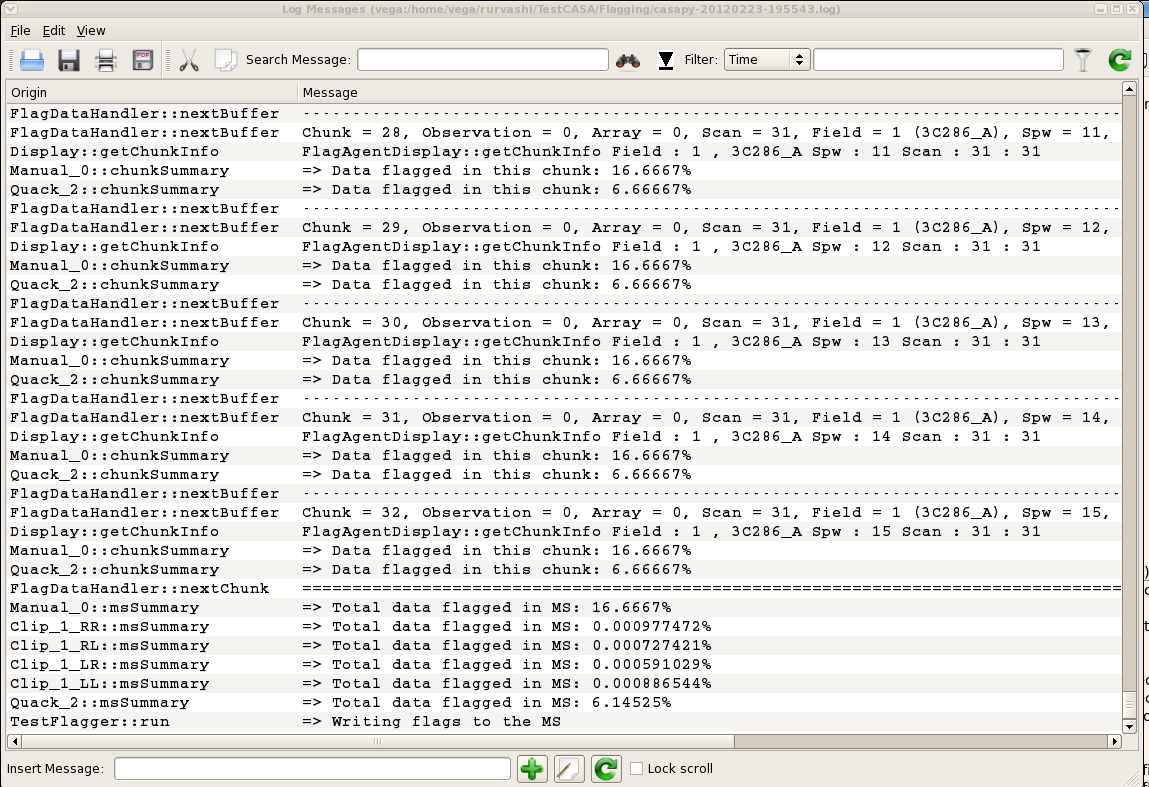
\includegraphics[scale=0.7]{flag.screenshot.logger.png}
\caption{Example of runtime logger summary of flag counts per agent}
\end{figure}

Flag count dictionaries : {\red verbatim output of part of one...}



\subsubsection{Flag Reports/Views}

Here are some examples of flag report displays on two datasets.
\begin{enumerate}
\item Percentage of data flagged vs frequency : To assess how much usable data is present in each spectral-window, for later processing, and imaging sensitivity-estimates.
\item Percentage of data flagged vs antenna-position : To assess whether the RFI is restricted to only some antennas and therefore may be local.
\item Percentage of data flagged vs baseline-length : To assess expected sensitivities for different spatial scales, since local RFI correlates better on shorter baselines than longer ones.
\end{enumerate}

\subsubsection{Data Display + action='calculate'}
In order to visualize some of the RFI present in the data, and to verify if flagging
commands are having the desired effect,  there is an option to 
visualize the data and flags at run-time, and navigate between baselines in the 
current chunk, as well as in the forward-direction across scans and spws.   

The intended usage of the display is to run the flagger on small subsets of the data (sub-selections)
with action='calculate', and display='data', and inspect the flagging results. 
An option to quit at any stage allows the user to change input parameters and try again until the
desired flagging results are obtained.  Then, the display can be turned off,
action set to 'apply', and the program run again on a larger section of the
data.


\subsection{Flagging Calibration-Tables}

\subsubsection{Ability to flag the new Calibration Table format}

The new Calibration Table format can be handled by the tasks flagdata, flagcmd and the
AgentFlagger tool in a
transparent way, just like a Measurement Set Table. If the calibration table was created before
CASA 4.1, the cal table handler will create a dummy OBSERVATION column and OBSERVATION
sub-table in the input calibration table to adapt it to the new cal table format. There is
limited support for older cal tables, therefore we recommend the user to re-create his/her
calibrations using CASA 4.1 before running flagdata.

There is an open-time check that inspects the table type and uses the appropriate FlagDataHandler
implementation for all the I/O operations:


\begin{verbatim}
CASA <2>: flagdata('X7ef.tsys', mode='unflag')
\end{verbatim}

\begin{verbatim}

CASA <2>: af.open('X7ef.tsys')
INFO	AgentFlagger::open	Table type is Calibration
  Out[2]: True

\end{verbatim}

Support for the new Calibration Table format has been introduced
transparently, so it is possible to flag them using any of the already available
modes for Measurement Sets. However, due to the nature of the data in
calibration tables, it only makes sense to use the following flag agent groups:

\begin{enumerate}

\item Auto-flagging (outliers detection) agents: clip, tfcrop, rflag:

\begin{verbatim}
# Using the flagdata task
flagdata('X7ef.tsys',mode='clip',clipzeros=True,clipminmax=[0.,600.],datacolumn='FPARAM' )
\end{verbatim}
 
\begin{verbatim}
# Using the agentflagger tool
af.open('X7ef.tsys')
af.selectdata()
agentClip={'mode':'clip','clipzeros':True,'clipminmax':[0.,600.],'datacolumn':'FPARAM'}
af.parseagentparameters(agentClip)
af.init()
af.run()
af.done()

\end{verbatim}

\item Manual flagging (meta-data selections like antenna/time-range):

\begin{verbatim}
# using the flagdata task
flagdata('X7ef.tsys', antenna='DV09')
\end{verbatim}

\begin{verbatim}
# Using the agentflagger tool
af.open('X7ef.tsys')
af.selectdata()
agentManual={'mode':'manual','antenna':'DV09'}
af.parseagentparameters(agentManual)
af.init()
af.run()
af.done() 

\end{verbatim}

\item Auxiliary modes: unflag, summary, display

\begin{verbatim}
# using the flagdata task
flagdata('X7ef.tsys', mode='summary', spwchan=True)

\end{verbatim}

\begin{verbatim}
# using the agentflagger tool
af.open('X7ef.tsys')
af.selectdata()
agentSummary={'mode':'summary', 'spwchan':True}
af.parseagentparameters(agentSummary)
af.init()
summary = af.run()
af.done()

\end{verbatim}

\end{enumerate}

Notice that the parameters names and types are the same as described in the
flagdata command-line help.

\subsubsection{Supported columns and expressions}

\begin{enumerate}

\item For the autoflagging agents (clip, tfcrop, rflag) it is possible to
choose the column to operate with, using the 'datacolumn' parameter, being 'FPARAM',
'CPARAM' and 'SNR' the currently supported columns. The given column will be validated and the 
correct one will be chosen based on the type of input:

\begin{verbatim}
# giving the correct datacolumn in the task
flagdata(vis='cal.fewscans.bpass', mode='clip', datacolumn='CPARAM', clipminmax=[0.,6.],clipzeros=True)

# using the default datacolumn in the agentflagger tool
af.open('cal.fewscans.bpass')
af.selectdata()
af.parseclipparameters(clipminmax=[0.,6.],datacolumn='CPARAM', clipzeros=True)
INFO    AgentFlagger::parseAgentParameters  Validating data column CPARAM based on input type
INFO    AgentFlagger::parseAgentParameters  Will use data column CPARAM
af.init()
af.run()
af.done()

\end{verbatim}

There is no default data column for cal tables. The task has DATA as the default for MSs. Once the
framework has detected the input to be a cal table, it will try to use the given data column. If that
does not exist (such as DATA), it will try to use FPARAM, then CPARAM. If none of the them exist, it
will exit with an error.

\begin{verbatim}
# using the flagdata task
flagdata(vis='cal.fewscans.bpass', mode='clip', clipminmax=[0.,6.])

# using the default datacolumn in the agentflagger tool
...
af.parseclipparameters(clipminmax=[0.,6.])
INFO    AgentFlagger::parseAgentParameters  Validating data column DATA based on input type
WARN    AgentFlagger::validateDataColumn    Only FPARAM, CPARAM and SNR are supported for cal tables
INFO    AgentFlagger::parseAgentParameters  Will use data column CPARAM
...
\end{verbatim}

\item Only for the autoflagging modes, it is also possible to choose the element of interest to inspect for
flagging, through the correlation parameter, specifying a list of comma-separated
elements or '' to select all the elements (which is also the default). If the CPARAM
datacolumn is used, the default correlation will be ABS\_ALL because this column contains 
complex data. For the other two supported columns (FPARAM,SNR), the default will fall 
back to REAL\_ALL.

When flagging using mode RFlag, it is important to notice that RFlag mixes the data from 
all the solutions (similar to the parallel and cross-hand correlation products in an MS) to 
determine the flagging thresholds. If some of the solutions have higher ranges than others, 
they will dominate the algorithm, thus showing results only for the higher ones. 
We recommend that the usual way to proceed is to run flagdata using only the parallel-hand 
correlation products (or analogous for cal tables) and then extend it to the cross-hand 
correlation products to obtain the correct results. 


\begin{verbatim}

agentClip={'mode':'clip',clipminmax':[0.,600.],'datacolumn':'FPARAM','correlation':'Sol1'}
af.parseagentparameters(agentClip)
af.init()
...
INFO	Clip::setAgentParameters	Visibility expression is REAL SOL1

agentClip={'mode':'clip','clipminmax':[0.,600.],'datacolumn':'CPARAM','correlation':''}
af.parseagentparameters(agentClip)
af.init()
...
INFO	Clip::setAgentParameters	Visibility expression is ABS SOL1,SOL2

\end{verbatim}

\begin{verbatim}

agentClip={'mode':'clip','clipminmax':[0.,6.]}
af.parseagentparameters(agentClip)
AgentFlagger::parseAgentParameters  Validating data column DATA based on input type
AgentFlagger::validateDataColumn    Only FPARAM, CPARAM and SNR are supported for cal tables
AgentFlagger::parseAgentParameters  Will use data column CPARAM
af.init()
...
INFO    Clip::setAgentParameters     Visibility expression is ABS SOL1,SOL2,SOL3,SOL4

\end{verbatim}

\end{enumerate}

\subsubsection{Meta-Data selection}

As far as meta-data selection is concerned, we are bounded to what MSSelection
interface for Calibration Tables offers (currently field, scan, time, spw, antenna
and observation selections). There are two ways to apply meta-data selections that can be used
independently or combined together:

\begin{enumerate}

\item FlagDataHandler selection (global): Create a sub-table with the selection
to be used by all the agents. The data selection parameters have to be parsed
through the selectdata() method of the AgentFlagger tool:

\begin{verbatim}
# using the flagdata task
flagdata(vis='X7ef.tsys', field='TW Hya')

# using the agentflagger tool
af.open('X7ef.tsys')
af.selectdata(field='TW Hya')
agentManual={'mode':'manual'}
af.parseagentparameters(agentManual)
af.init()
af.run()
af.done() 
		
\end{verbatim}

\item Agent selection (specific to each agent): To restrict the rows that each
agent inspect for flagging. The data selection parameters can be parsed as
normal agent parameters:

\begin{verbatim}
# using the flagdata task
flagdata(vis='X7ef.tsys', antenna='DV09')

# using the agentflagger tool
af.open('X7ef.tsys')
af.selectdata()
agentManual={'mode':'manual','antenna':'DV09'}
af.parseagentparameters(agentManual)
af.init()
af.run()
af.done() 
		
\end{verbatim}

\item Combined selection : To iterate only through a global selection, and at the
same time have each agent inspecting a particular group of rows for flagging:

\begin{verbatim}
# using the flagdata task
flagdata(vis='X7ef.tsys', field='TW Hya', antenna='DV09')

# using the agentflagger tool
af.open('X7ef.tsys')
af.selectdata(field='TW Hya')
agentManual={'mode':'manual','antenna':'DV09'}
af.parseagentparameters(agentManual)
af.init()
af.run()
af.done() 
		 
\end{verbatim}

\end{enumerate}

\subsubsection{Combining several modes in a single run}

As with MeasurementSet tables, the re-factored flagger framework allows running
several flagging agents at the same time, to reduce I/O overhead,  for instance:

\begin{enumerate}

\item Combination of tfcrop and rflag:

\begin{verbatim}
# using the flagdata task
flagdata(vis='cal.fewscans.bpass', mode='list', 
         inpfile=["mode='rflag' datacolumn='CPARAM' correlation='Sol1'",
                   mode='tfcrop' datacolumn='CPARAM' correlation='Sol1'"])

# using the agentflagger tool
af.open('cal.fewscans.bpass')
af.selectdata()
agentRflag={'mode':'rflag','datacolumn':'CPARAM','correlation':'Sol1'}
agentTfcrop={'mode':'tfcrop','datacolumn':'CPARAM','correlation':'Sol1'}
af.parseagentparameters(agentRflag)
af.parseagentparameters(agentTfcrop)
af.init()
af.run(writeflags=True)
af.done()

\end{verbatim}

\begin{figure}
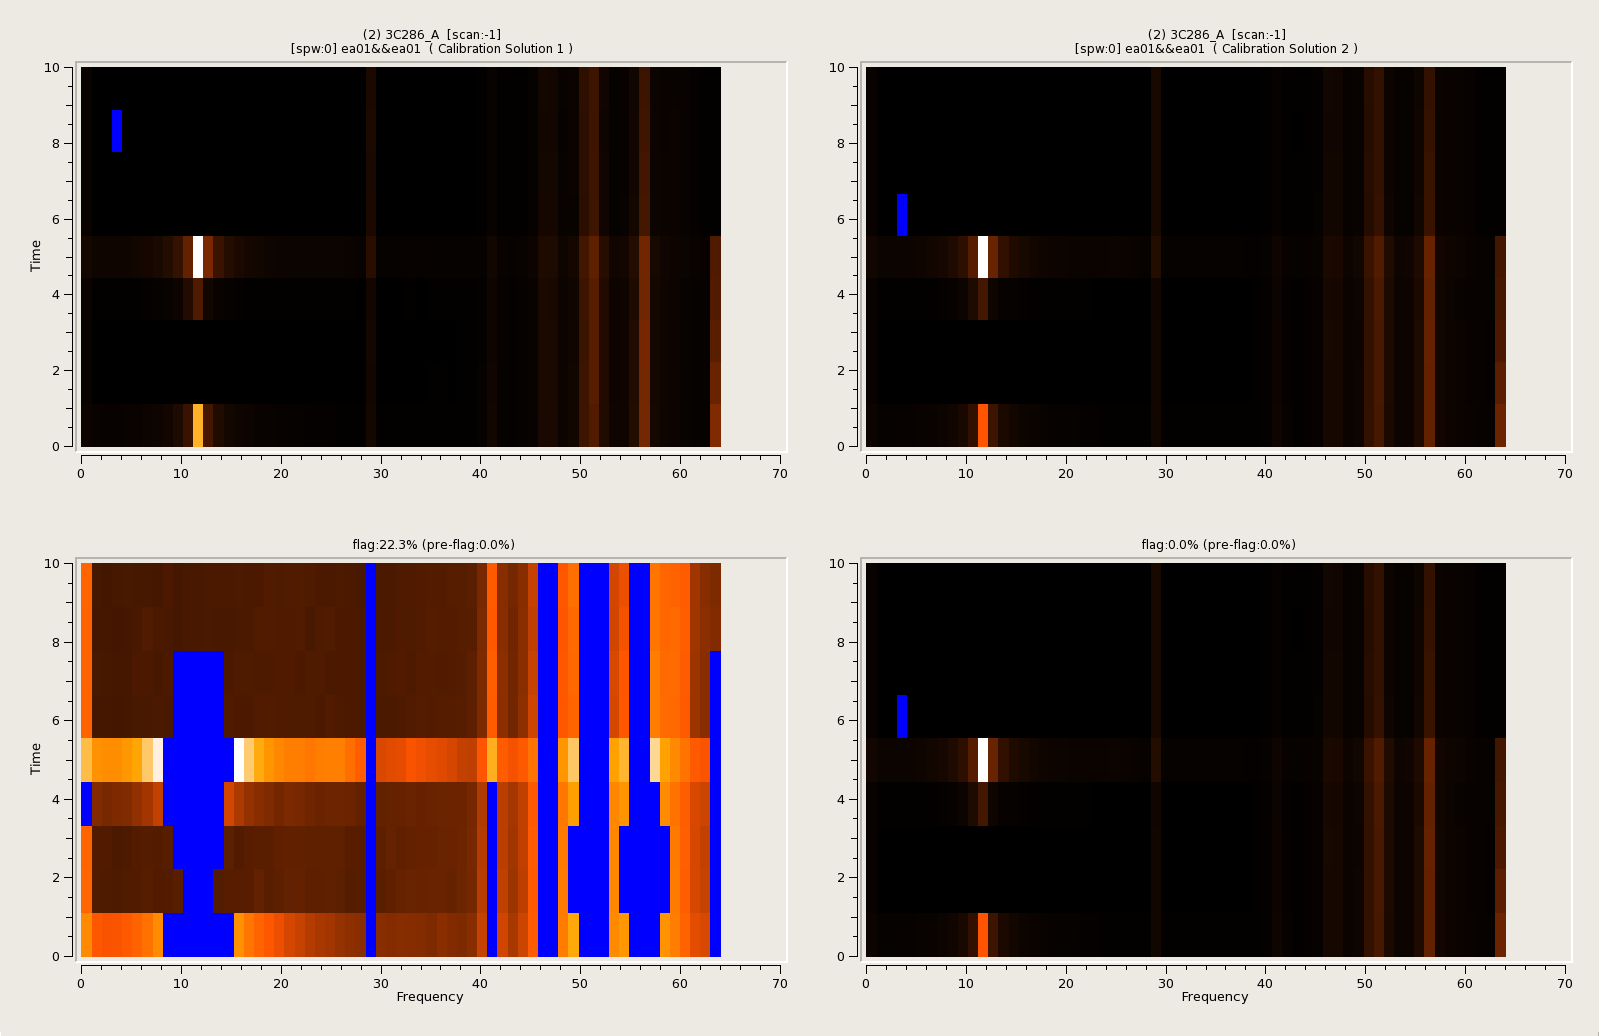
\includegraphics[scale=0.5]{CalTable-RFlag+TFCrop.png}
\caption{Rflag and TFCrop agents combined in a single run applied on a EVLA
band-pass calibration table}
\label{Fig:EVLA Band Pass Cal Table RFlag+TFCrop applied combined}
\end{figure}

\item Unflag + Clip + Display

\begin{verbatim}
# using the flagdata task
flagdata(vis='X7ef.tsys', mode='unflag')
flagdata(vis='X7ef.tsys', mode='clip',clipminmax=[0.,600.],datacolumn='FPARAM',correlation='Sol1',
         display='data')

# using the agentflagger tool
af.open('X7ef.tsys')
af.selectdata()
agentUnflag={'mode':'unflag'}
agentClip={'mode':'clip','clipminmax':[0.,600.],'datacolumn':'FPARAM','correlation':'Sol1'}
agentDisplay={'mode':'display','datadisplay':True}
af.parseagentparameters(agentUnflag)
af.parseagentparameters(agentClip)
af.parseagentparameters(agentDisplay)
af.init()
af.run(writeflags=True)
af.done()

\end{verbatim}

\begin{figure}
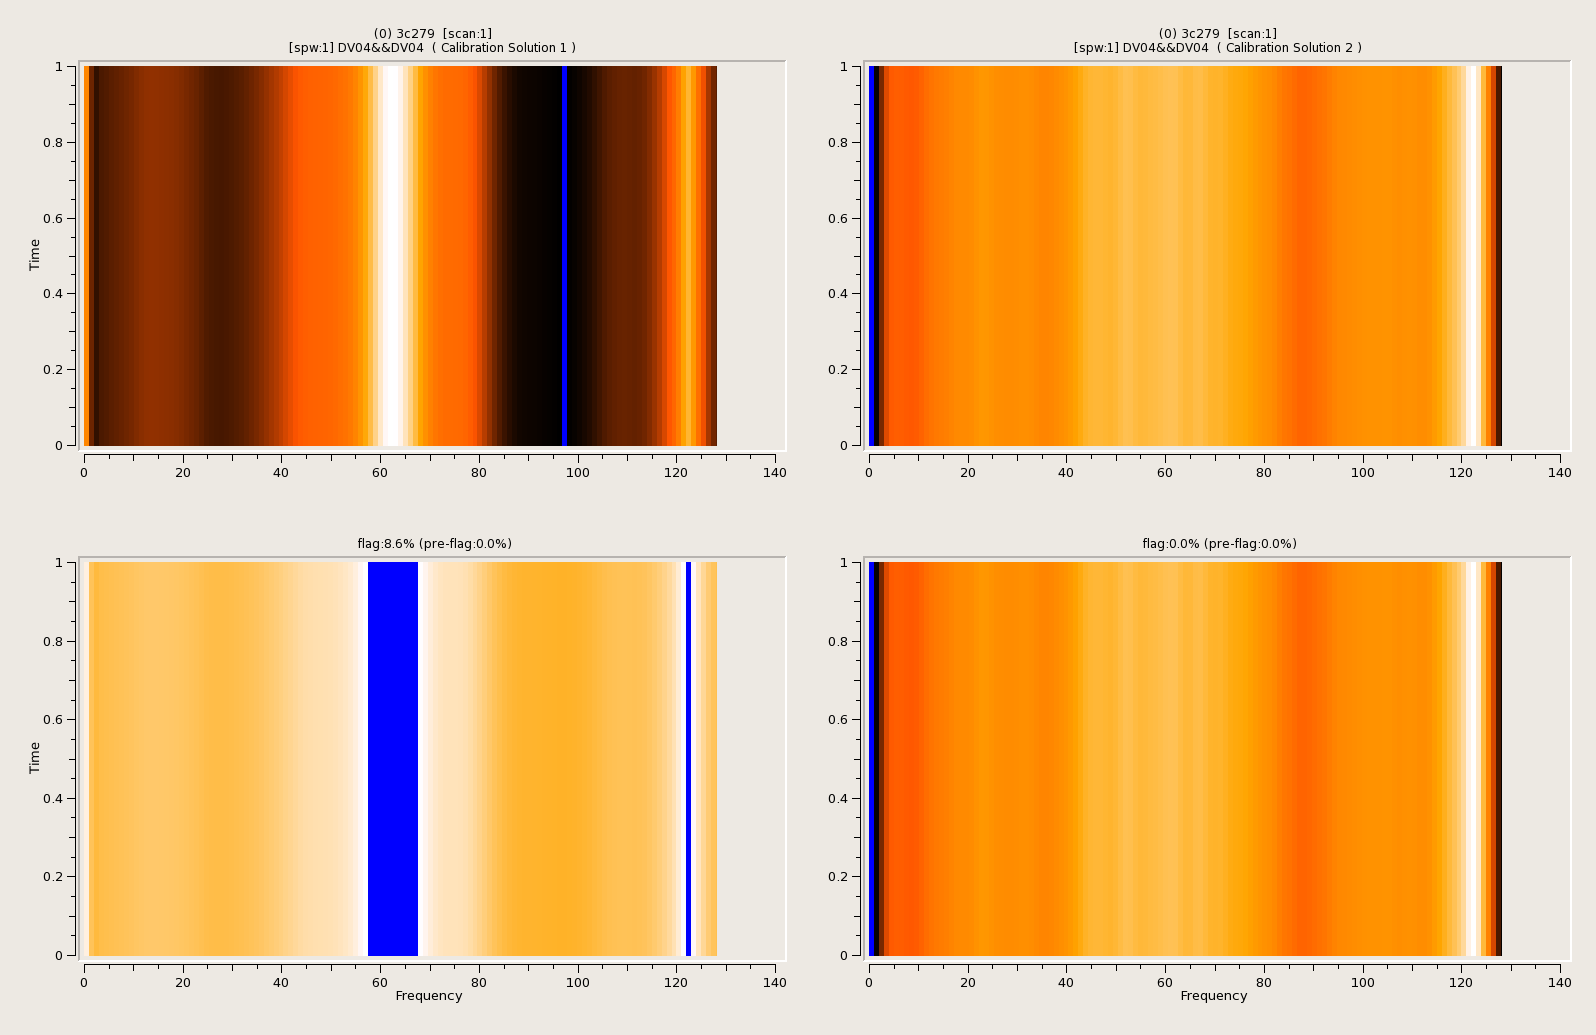
\includegraphics[scale=0.5]{CalTable-Clip.png}
\caption{Clipping agent operating on ALMA TSys CalTable (TW Hya Science
Verification data)}
\label{Fig:TW Hya CalTable Clip}
\end{figure}

\item Unflag + Manual Selection (channel edges) + Summary
\begin{verbatim}
# using the flagdata task
flagdata(vis='X7ef.tsys', mode='unflag')
flagdata(vis='X7ef.tsys', spw='*:0~9;118~127', display='data')

# using the agentflagger tool
af.open('X7ef.tsys')
af.selectdata()
agentUnflag={'mode':'unflag'}
agentManual={'mode':'manual','spw':'*:0~9;118~127'}
agentDisplay={'mode':'display','datadisplay':True}
af.parseagentparameters(agentUnflag)
af.parseagentparameters(agentManual)
af.parseagentparameters(agentDisplay)
af.init()
af.run(writeflags=True)
af.done() 

\end{verbatim}

\begin{figure}
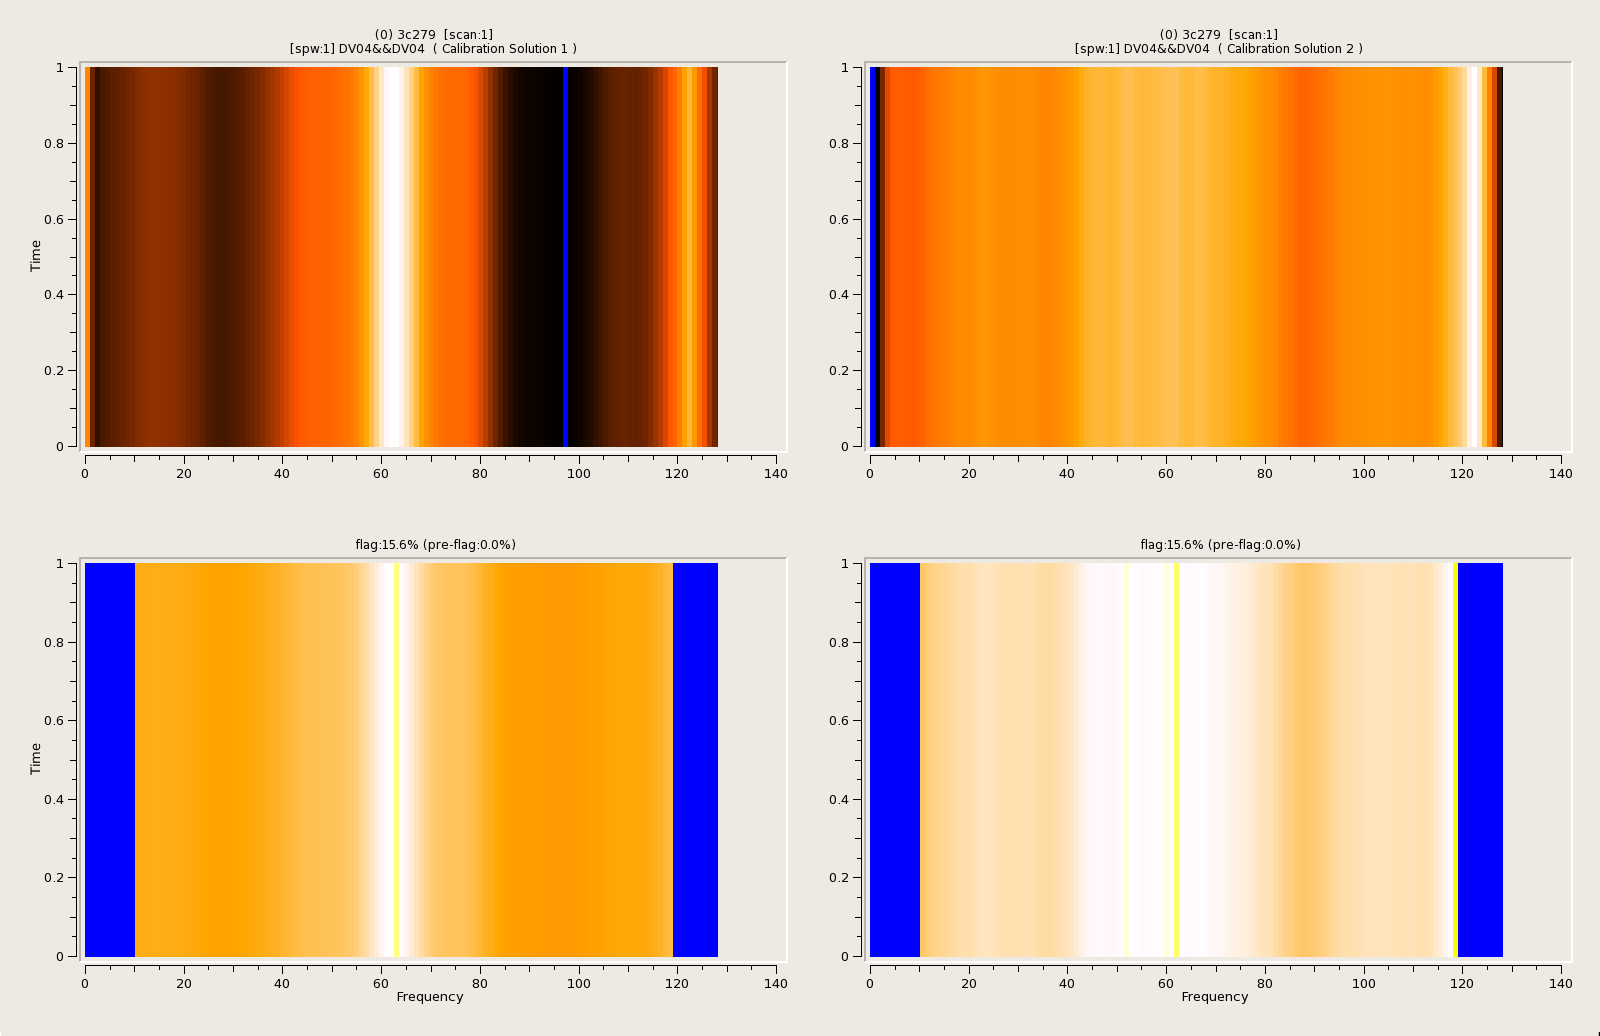
\includegraphics[scale=0.5]{CalTable-MultipleChannel.png}
\caption{Clipping agent operating on ALMA TSys CalTable (TW Hya Science
Verification data)}
\label{Fig:TW Hya CalTable Clip}
\end{figure}

\item Unflag + Manual Selection (antenna) + Summary
\begin{verbatim}
# using the flagdata task
flagdata(vis='X7ef.tsys', mode='unflag')
flagdata(vis='X7ef.tsys', antenna='DV09')

# next command will return the summary with baseline counting
flagdata(vis='X7ef.tsys', mode='summary', basecnt=True)

# using the agentflagger tool
af.open('X7ef.tsys')
af.selectdata()
agentUnflag={'mode':'unflag'}
agentManual={'mode':'manual','antenna':'DV09'}
agentSummary={'mode':'summary'}
af.parseagentparameters(agentUnflag)
af.parseagentparameters(agentManual)
af.parseagentparameters(agentSummary)
af.init()
summary = af.run(writeflags=True)
af.done() 

CASA <12>: summary
  Out[12]: 
{'nreport': 2,
 'report0': {'antenna': {'DV04': {'flagged': 0.0, 'total': 14336.0},
                         'DV06': {'flagged': 0.0, 'total': 14336.0},
                         'DV07': {'flagged': 0.0, 'total': 14336.0},
                         'DV08': {'flagged': 0.0, 'total': 14336.0},
                         'DV09': {'flagged': 14336.0, 'total': 14336.0},
                         'DV10': {'flagged': 0.0, 'total': 14336.0},
                         'PM01': {'flagged': 0.0, 'total': 14336.0},
                         'PM02': {'flagged': 0.0, 'total': 14336.0},
                         'PM03': {'flagged': 0.0, 'total': 14336.0}},


\end{verbatim}

\end{enumerate}


\section{Frequently Asked Questions}\label{Sec:FAQ}

\subsection{Obtaining summaries per reason}
\begin{verbatim}

#########################################################################
#
#   Function to count statistics as a function of 'reason'
#   
#   Flag Zeros, and run TFCrop, gathering incremental summary statistics.
#
#########################################################################
def task_reason_stats(msname='',field='',spw='',writeflags=True):

    # Open the MS and select data
    af.open(msname=msname,ntime=100.0);
    af.selectdata(field=field, spw=spw);

    # Unflag (This is only for a demo)
    ag0 = {'apply':True, 'sequential':True, 'mode':'unflag'}
    af.parseagentparameters(ag0);

    # (1) Flag Zeros
    ag1 = {'apply':True,'sequential':True,'mode':'clip', 'clipzeros':True}
    af.parseagentparameters(ag1);
    # (2) Summary
    ag2 = {'apply':True,'sequential':True,'mode':'summary','name':'Zeros'}
    af.parseagentparameters(ag2);
    # (3) TFCrop
    ag3 = {'apply':True,'sequential':True,'mode':'tfcrop'}
    af.parseagentparameters(ag3);
    # (4) Summary
    ag4 = {'apply':True,'sequential':True,'mode':'summary', 'name':'TFCrop'}
    af.parseagentparameters(ag4);


    # Run all these agents, and get the combined-report.
    af.init();
    summary_stats_list = af.run(writeflags=writeflags);
    af.done();

    # Parse the output summary lists and extract only 'type==summary'
    ## Iterate through the list in the correct order. Do not follow default 'dictionary-key' ordering.
    summary_reps=[];
    for rep in range(0,summary_stats_list['nreport']):
        repname = 'report'+str(rep);
        if(summary_stats_list[repname]['type']=='summary'):
              summary_reps.append(summary_stats_list[repname]);

    # Step through the summary list and print a few things.
    ## SUBTRACT flag counts from previous agents, because the counts are cumulative.
    for ind in range(0,len(summary_reps)):

        flagcount = summary_reps[ind]['flagged'];
        totalcount = summary_reps[ind]['total'];
     
        # From the second summary onwards, subtract counts from the previous one :)
        if ( ind > 0 ):
             flagcount = flagcount - summary_reps[ind-1]['flagged'];

        print "Summary ", ind , "(" , summary_reps[ind]['name']  , ") :  Flagged : " , flagcount , " out 
of " , totalcount ;

    return summary_reps; 


##############################################

\end{verbatim}


\subsection{FLAG\_CMD sub-table vs flag-command text files}
See section \ref{Sec:FlagCmdLists}


\subsection{Will batch modes make the flagging faster?}

Batch operations will help only if data and flag I/O is shared between the flag commands.  
If commands touch different data-selections, running them together will not help.

\begin{enumerate}
\item The following sequence of operations will benefit from being run together, 
because they all access spw 9, clip and rflag read visibilities, and rflag and extend read flags:

mode='manual'  spw='9:0~3;61~63' \\
mode='clip'  clipminmix=[0.0, 1e+5] \\
mode='rflag'   spw='9' \\
mode='extend'  growtime=80.0   extendpols=True 

\item This is an example that will not benefit from the list mode : 

mode='manual'  spw='9:0~3;61~63' \\
mode='clip'  spw = '5'  clipminmix=[0.0, 1e+5] 

\end{enumerate}




\subsection{Comparison of RFI with 1s vs 10s integrations}
In order to reduce dataset sizes, data can be averaged during the observation. However, with integration-times of anything larger than few seconds, there is the risk of smearing out the RFI and losing a larger fraction of the data to RFI.   

The following is the result of a few autoflag tests on an L-Band D-config 7-hour dataset (G55.7+3.4), for which we have a version with 1sec integrations,a 10s averaged version (with and without pre-applying online flags).

%, and a set of flags created by hand on one of the 10sec averaged versions. 

Figures \ref{Fig:compare_1} and \ref{Fig:compare_2} show the percentage of data flagged per frequency-channel for the 1sec and 10sec datasets respectively, showing a few\% less data flagged in the 10sec dataset.  Figures \ref{Fig:compare_3} and \ref{Fig:compare_4} show the percentage flagged per antenna and scan (each scan is 1.5 minutes long), and show a difference of about 1\% in the amount of data flagged by 'rflag', indicating that there is no practical loss of data due to smearing out of the RFI during the 1sec-to-10sec averaging. 
Figure  \ref{Fig:compare_5} is the result of applying online flags on the 1-sec data before averaging to 10-sec and running rflag. Comparing with the previous plots, this saves about 1\% to 2\% of the flagged data. 

Figure  \ref{Fig:compare_6} shows plots of the un-calibrated data for the first two cases (1sec and 10sec), to demonstrate that 'rflag' has identified RFI correctly in both cases. Note that the 1-sec data were averaged for the purpose of plotting (after flagging).

These quick tests and summaries show that from the point of view of RFI-identification and flagging, there is no advantage of recording data at a 1-sec for D-Config and L-Band. In general, it should suffice if averaging rules follow time-smearing limits at any given configuration.

\begin{figure}
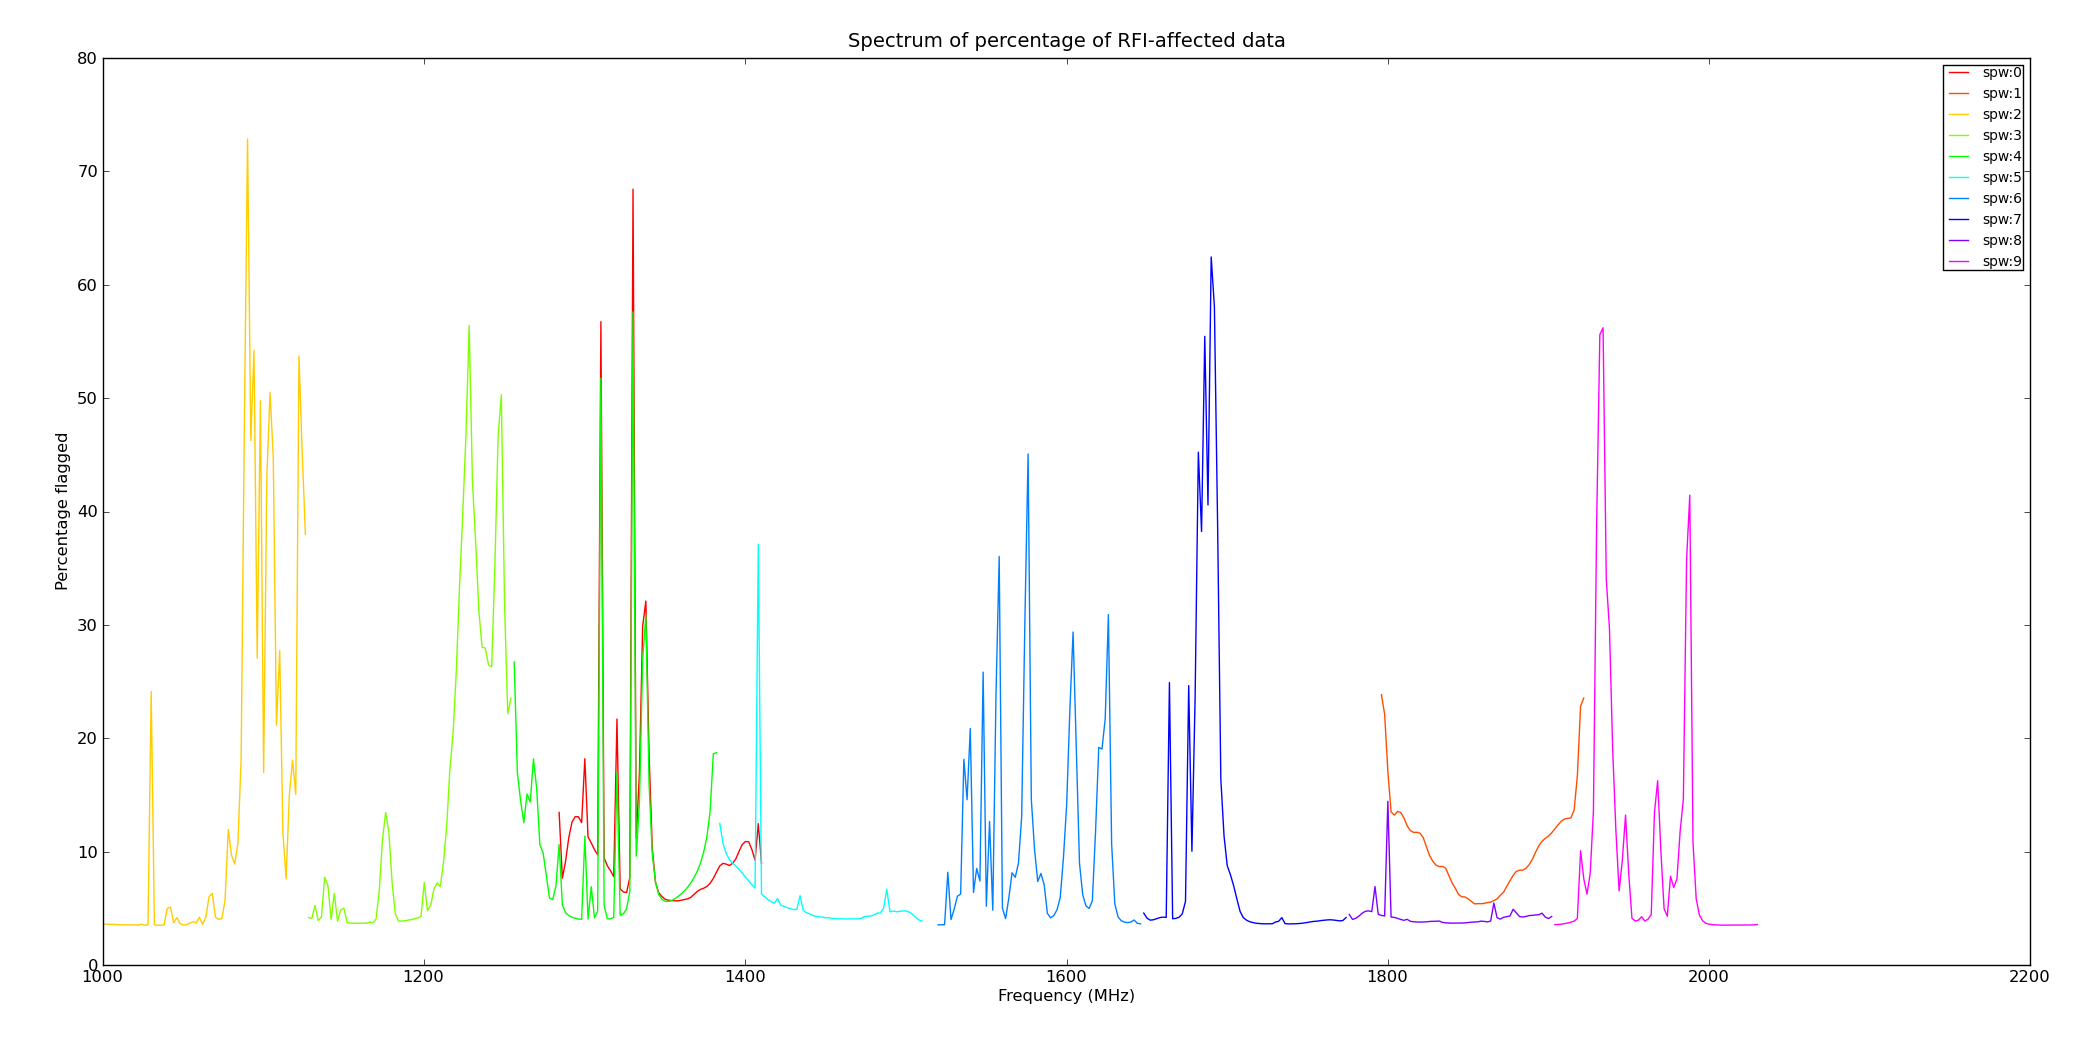
\includegraphics[scale=0.5]{plot.anttime.G55.1s.freqplot.png}
\caption{Plots of the percentage flagged per channel :  Dataset with 1sec timesteps.}
\label{Fig:compare_1}
\end{figure}

\begin{figure}
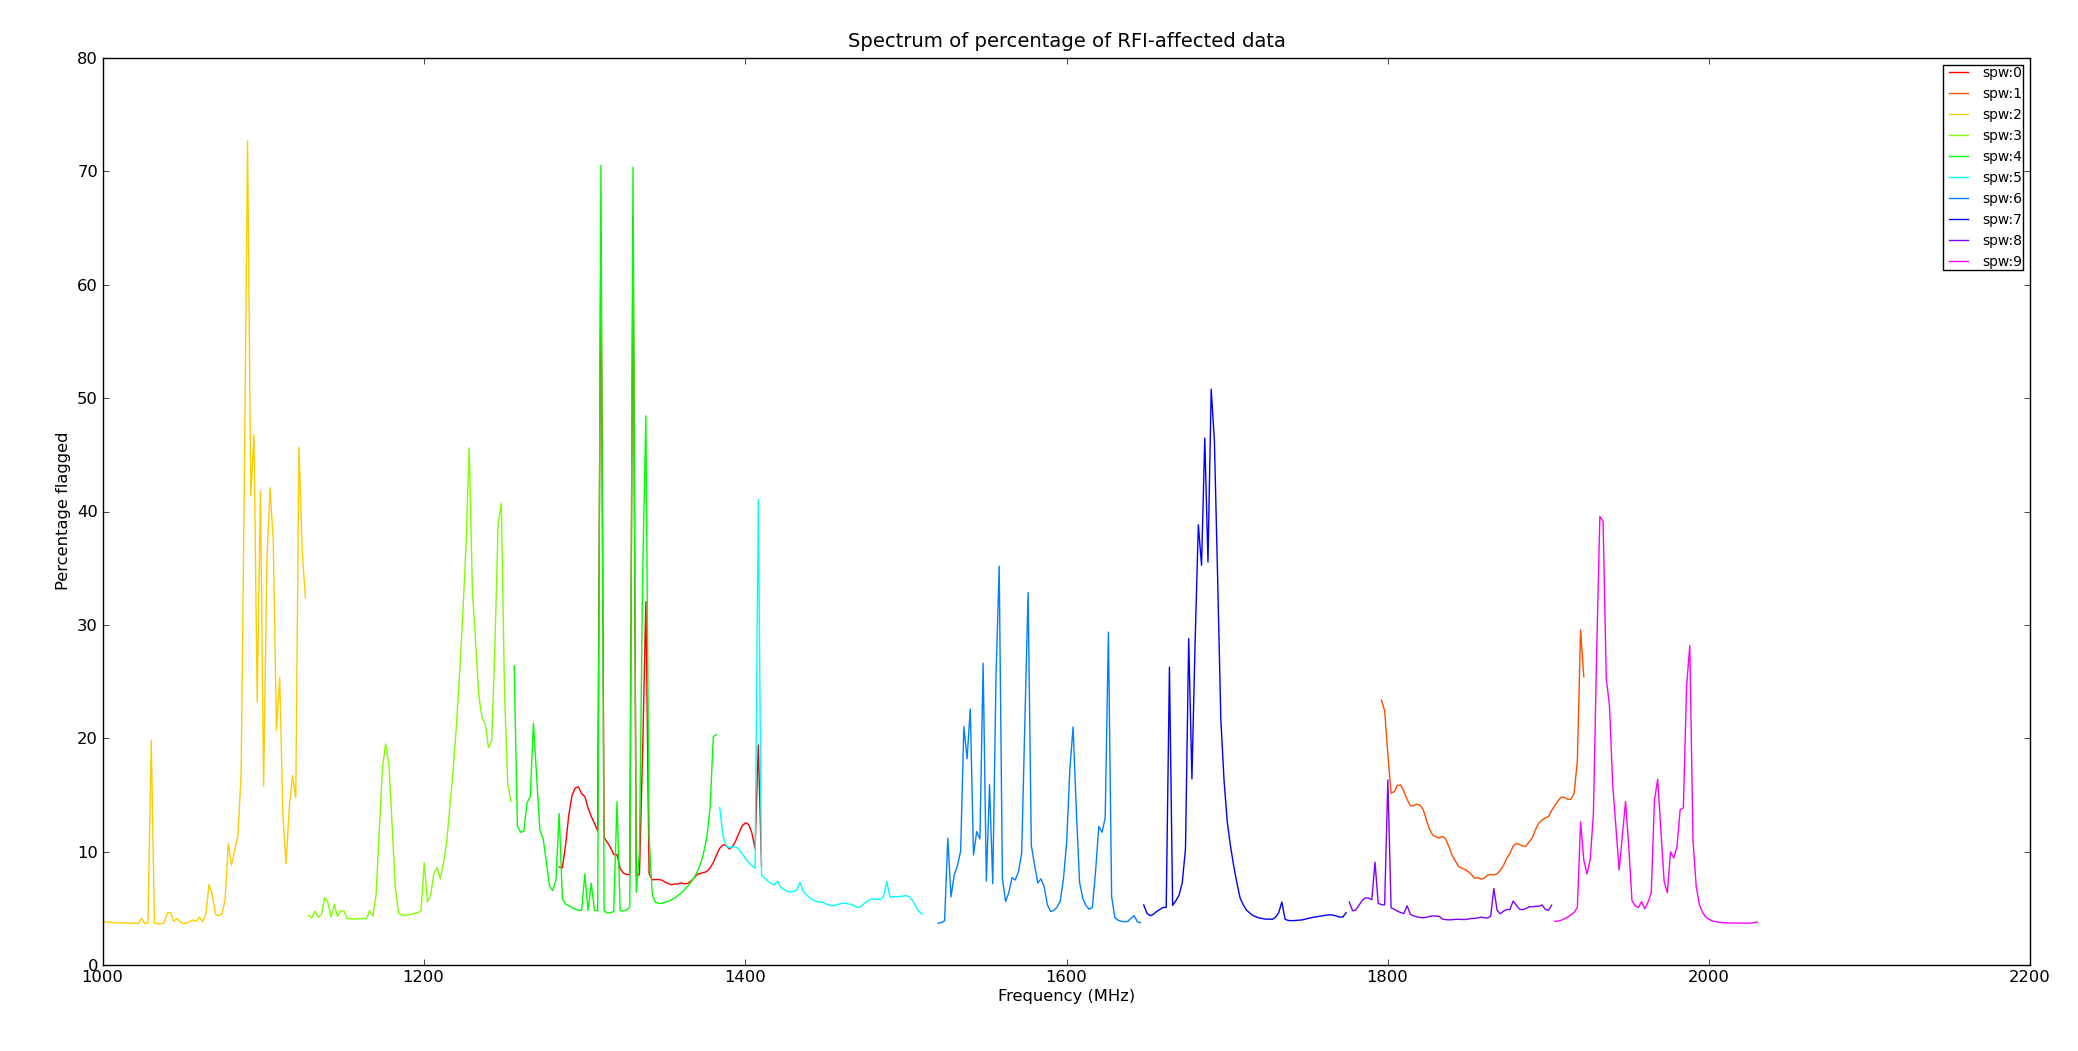
\includegraphics[scale=0.5]{plot.anttime.G55.averaged.10s.freqplot.png}
\caption{Plots of the percentage flagged per channel : Dataset with 10sec timesteps.}
\label{Fig:compare_2}
\end{figure}

\begin{figure}
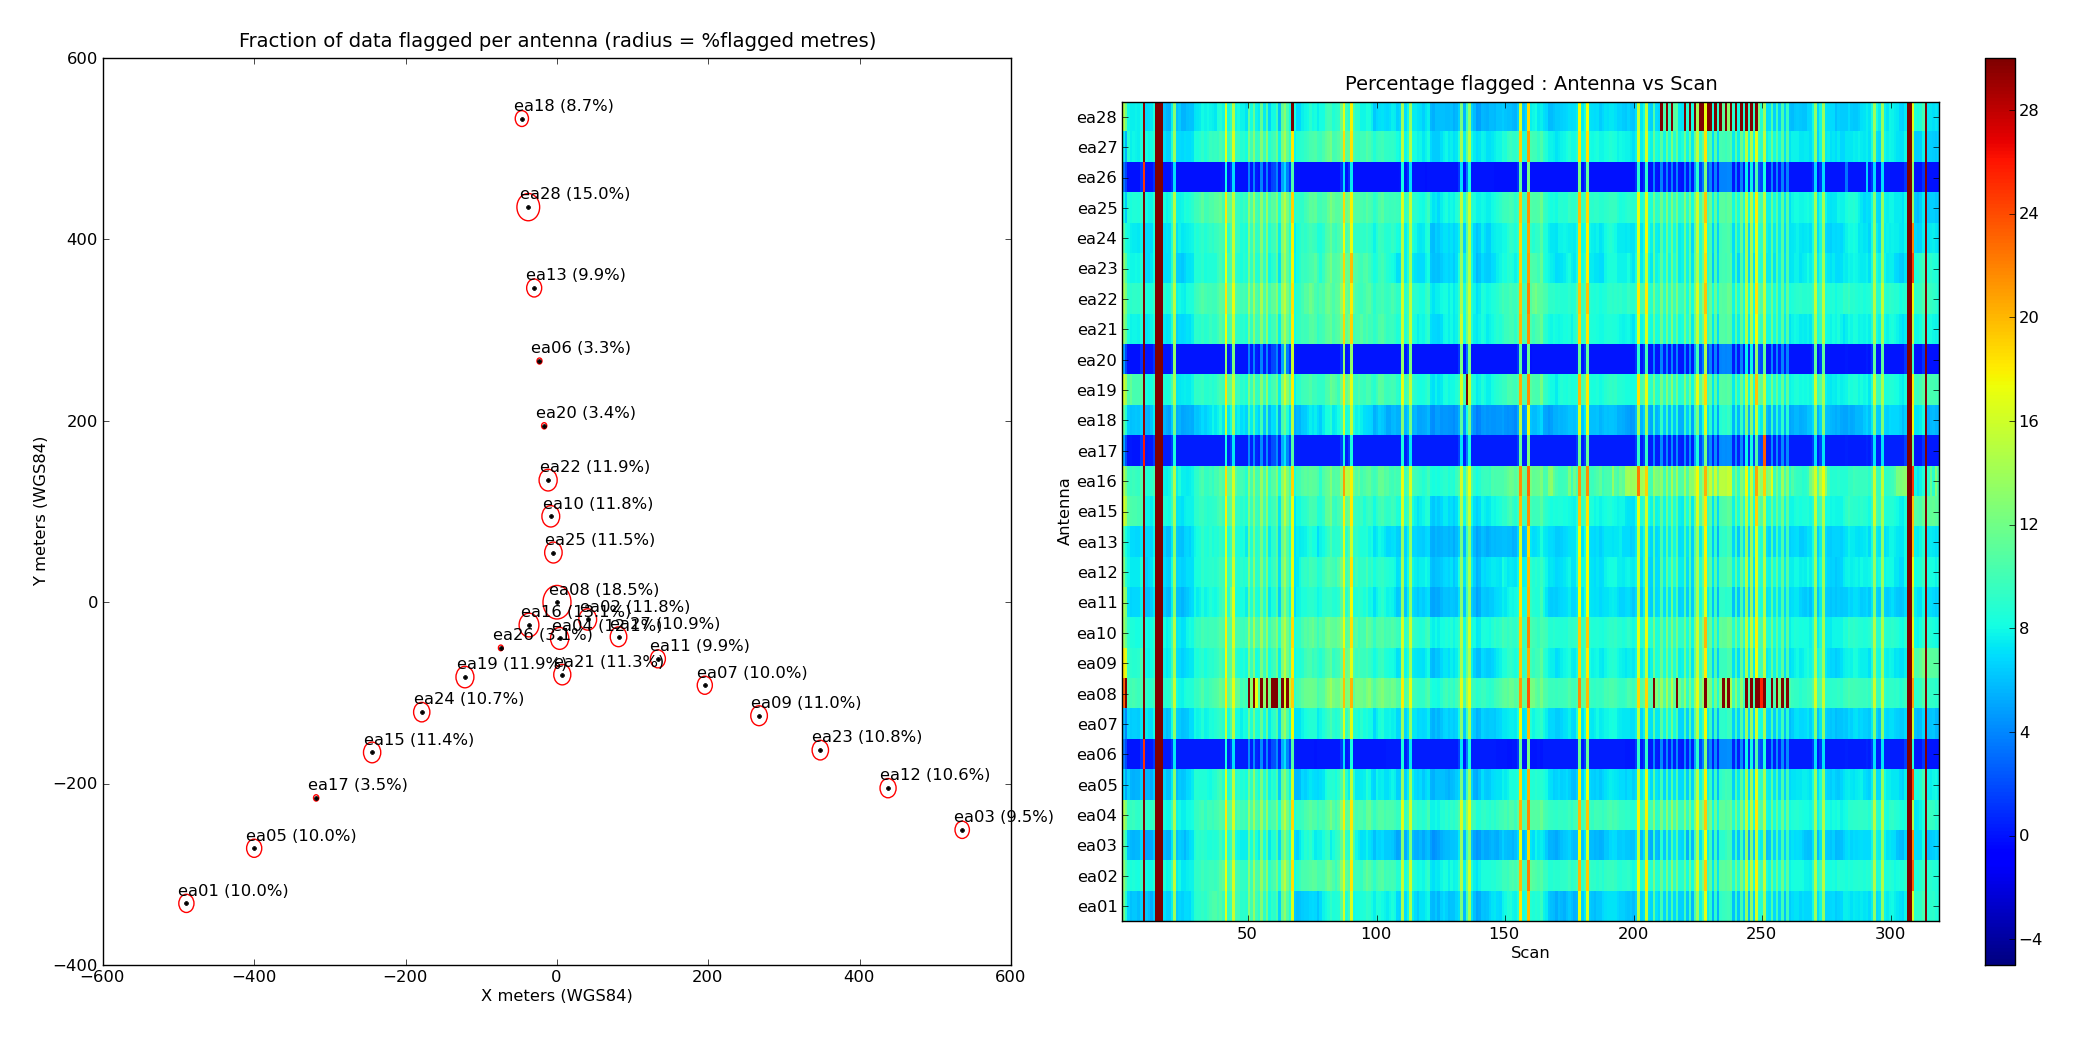
\includegraphics[scale=0.5]{plot.anttime.G55.1s.scanplot.png}
\caption{Dataset with 1sec timesteps : Plots of the percentage flagged per antenna and scan. Each scan is about 1.5 minutes long. Flagging includes online flags followed by rflag running per scan. The left panel shows the percentage flagged per antenna, over all scans.}
\label{Fig:compare_3}
\end{figure}

\begin{figure}
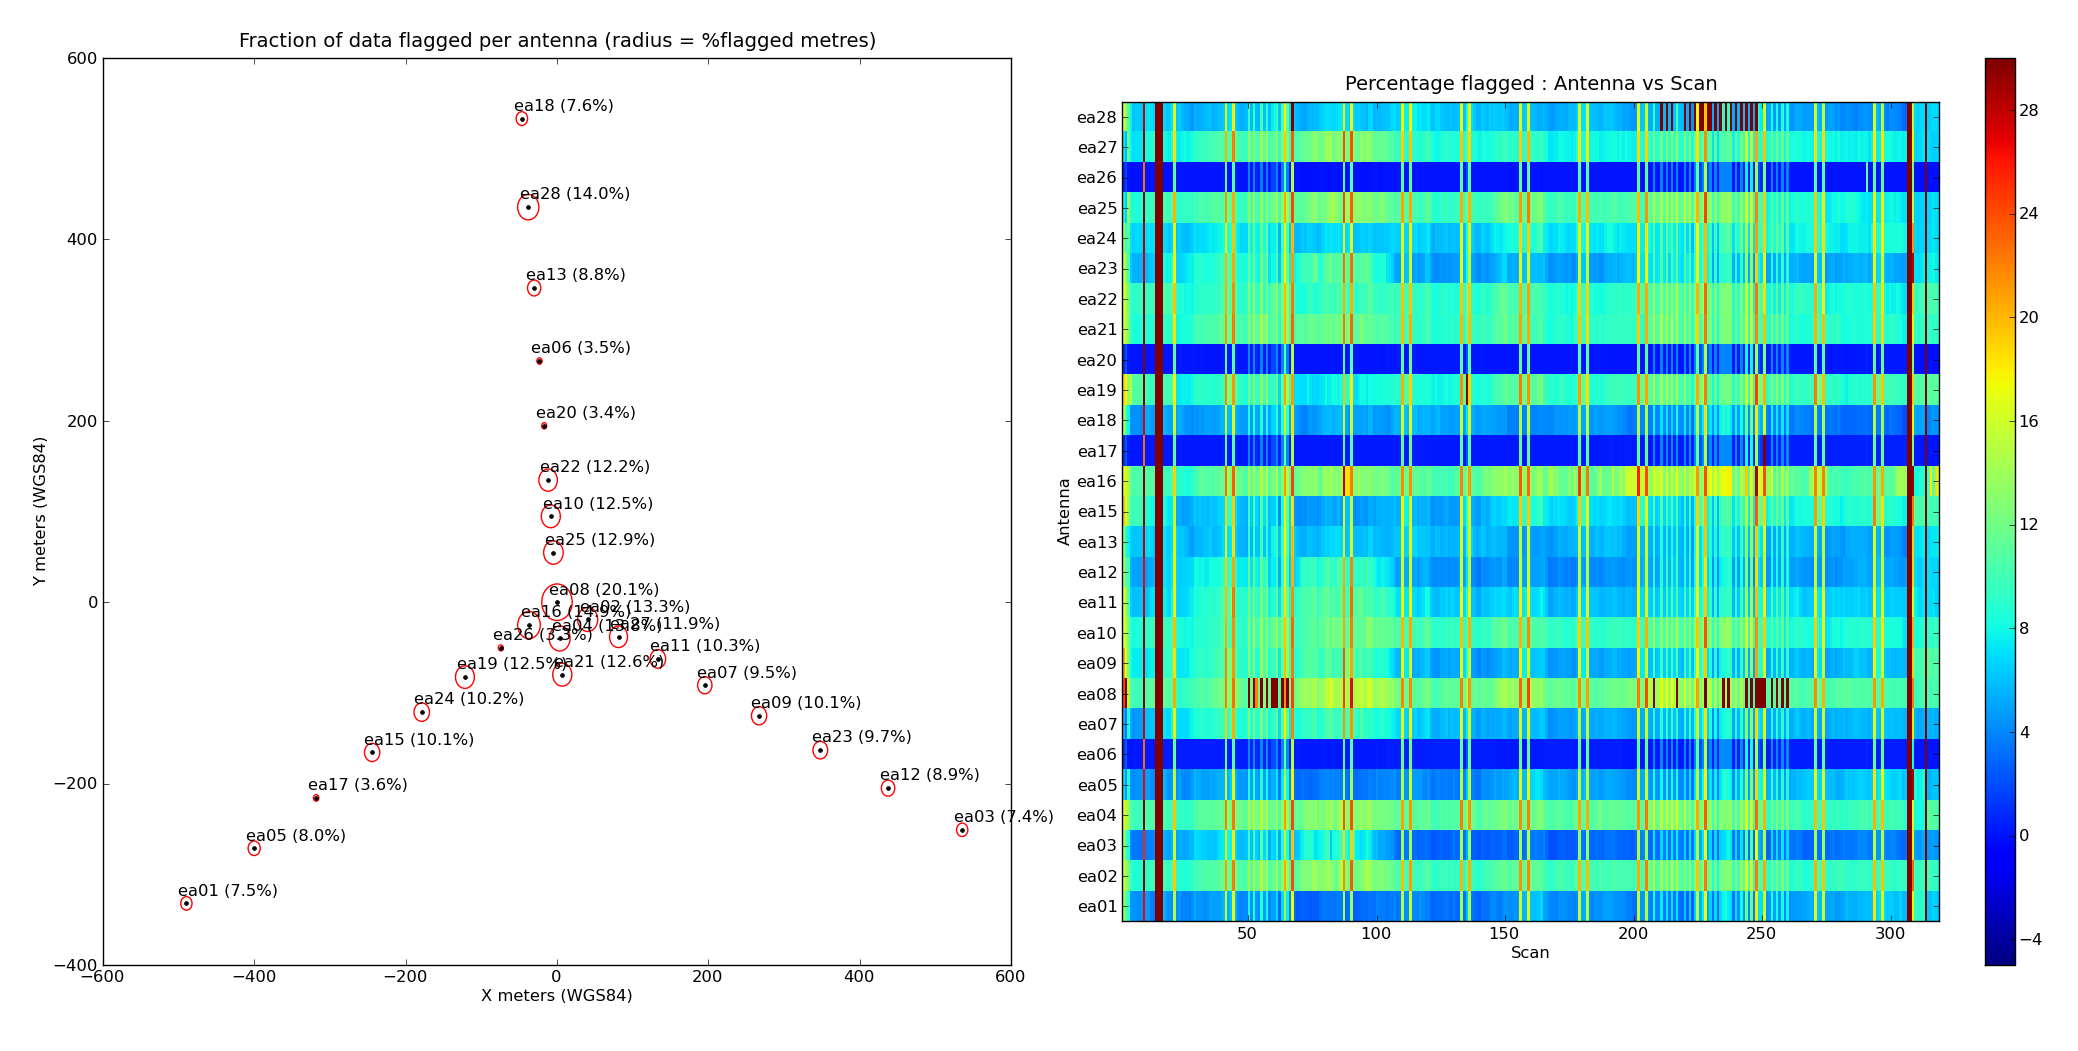
\includegraphics[scale=0.5]{plot.anttime.G55.averaged.10s.scanplot.png}
\caption{Dataset with 10sec timesteps : Plots of the percentage flagged per antenna and scan. Each scan is about 1.5 minutes long. Flagging includes online flags followed by rflag running per scan. The data was completely unflagged before averaging to 10sec, to simulate averaging within the correlator.}
\label{Fig:compare_4}
\end{figure}

\begin{figure}
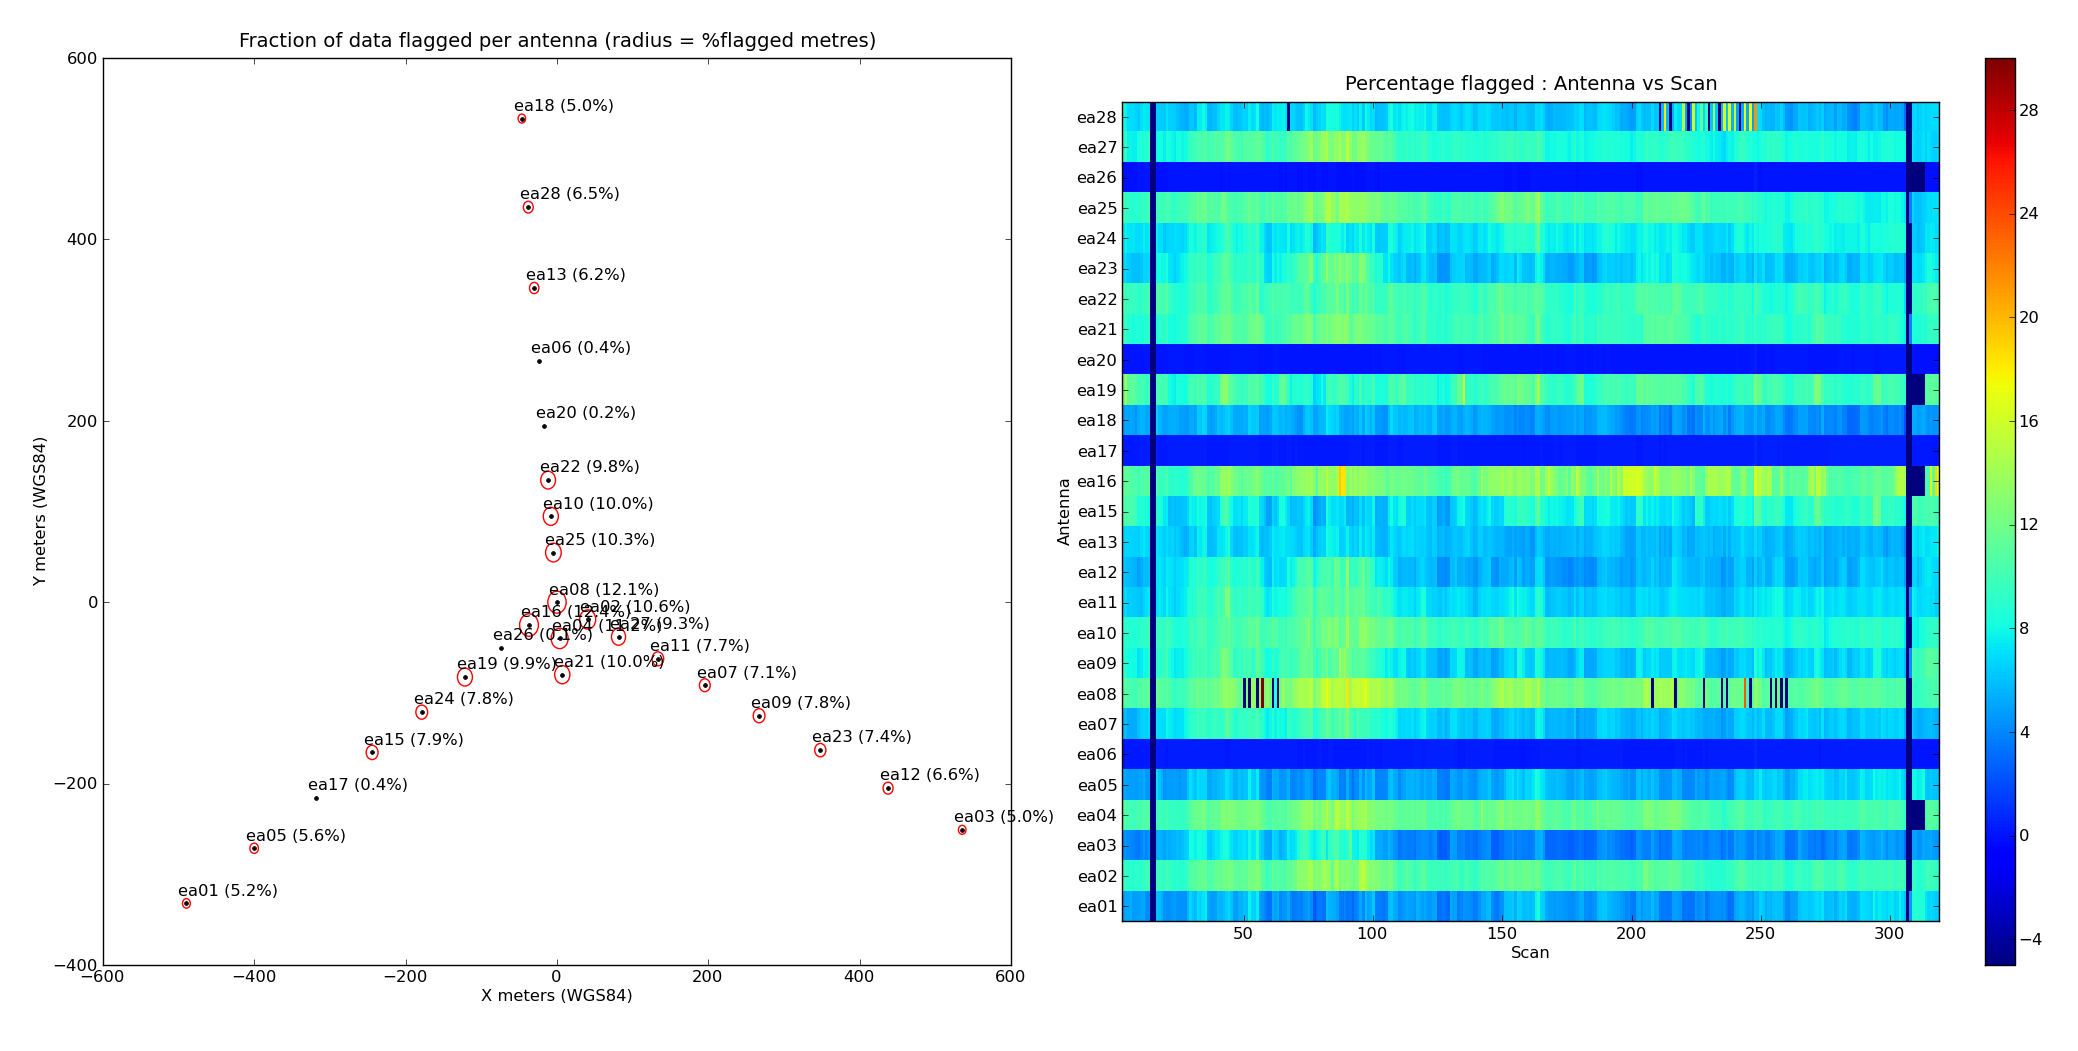
\includegraphics[scale=0.5]{plot.anttime.G55.10s.scanplot.png}
\caption{Dataset with 10sec timesteps, with online flags applied before averaging from 1sec to 10sec.  Plots of the percentage flagged per antenna and scan. Each scan is about 1.5 minutes long. Comparing with the previous two plots, again, there is very little gain (about 2\% of data) of applying online flags before averaging to 10sec. }
\label{Fig:compare_5}
\end{figure}


\begin{figure}
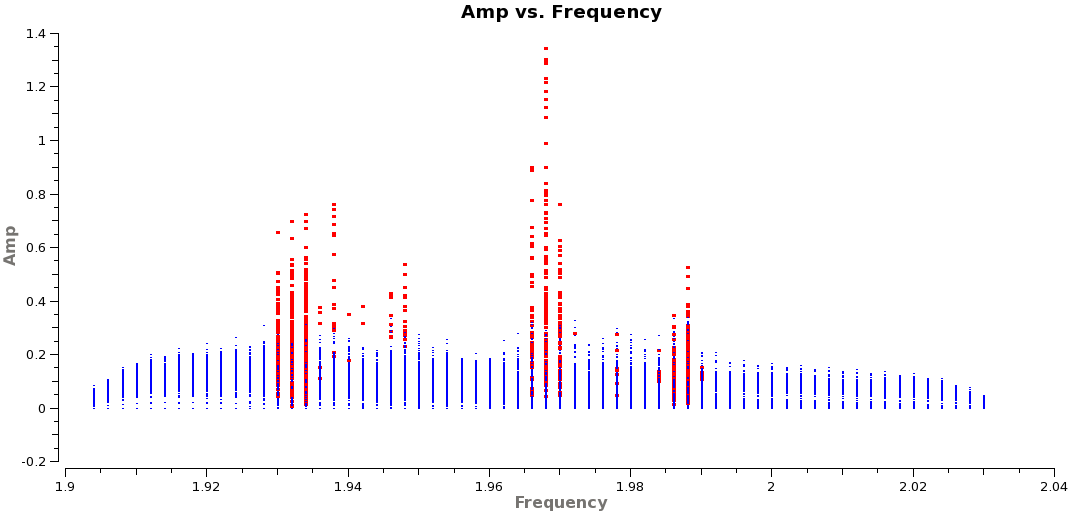
\includegraphics[scale=0.5]{plot.spectrum.ea11.spw9.1s.png}
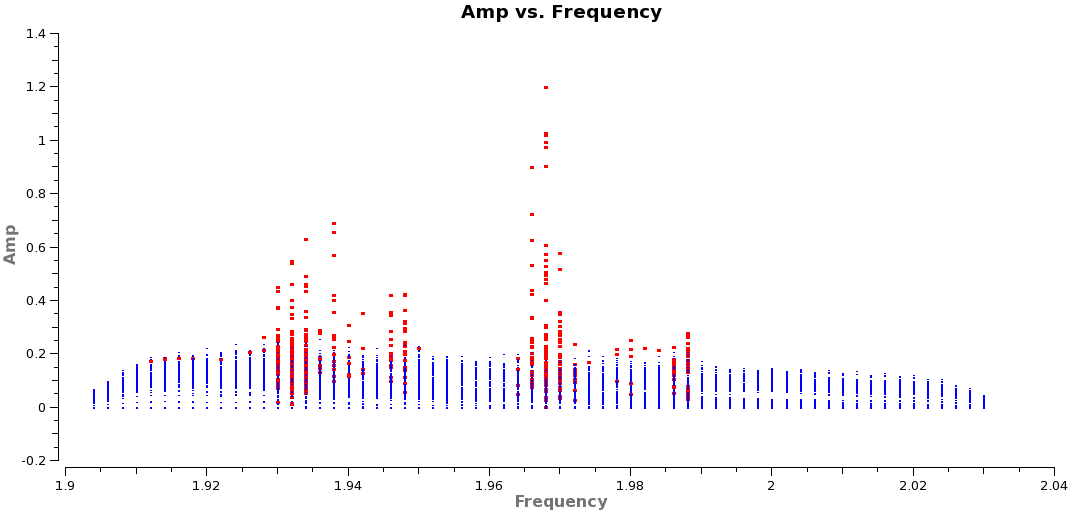
\includegraphics[scale=0.5]{plot.spectrum.ea11.spw9.avg10s.png}
\caption{Data amplitude vs frequency (flagged points are in red) for SPW=9, scan 7, and antenna EA11.  (FIRST) : Result of rflag run on 1sec timestep data, and averaged to 10s only during plotting.  (SECOND) : Result of rflag run on 10sec timestep data.}
\label{Fig:compare_6}
\end{figure}



\subsection{Comparison of autoflag methods}
What are the advantages and disadvantages?  What types of RFI are the defaults of tfcrop and 
rflag optimized for?  

\begin{figure}
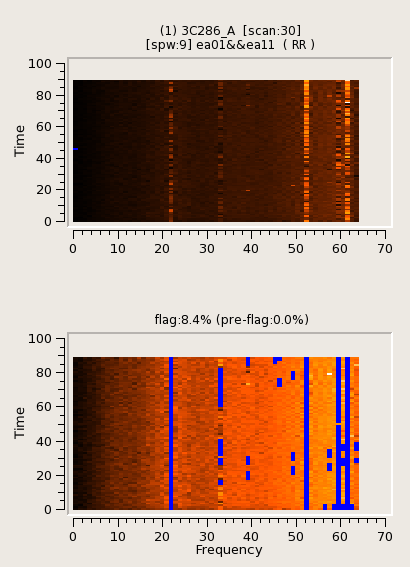
\includegraphics[scale=0.7]{rflag.before.after.png}
\caption{Example of rflag on narrow-band RFI}
\end{figure}



\subsection{Effect of Hanning-smoothing on RFI}
When does it help, when does it hurt.... 

\subsection{Is auto-flagging good-enough for imaging?}
A comparison of images and flag-summary counts,  with only autoflag runs, and with more careful hand-flagging. 








\end{document}


